\documentclass[12pt,a4paper,twoside]{ctexrep}
\usepackage{Alegreya}
\usepackage{AlegreyaSans}
\usepackage{DejaVuSansMono}
\usepackage{csquotes}
\usepackage{amsmath}             % Split equations
\usepackage{mathpazo}
\usepackage{fontspec}
\usepackage{fancyhdr}
\usepackage[explicit]{titlesec}
\usepackage{graphicx}
\usepackage[table]{xcolor}
\usepackage{pbox}
\usepackage{tikz}
\usepackage{listings}            % Code syntax highlighting
\usepackage{ctable}
\usepackage{multirow}
\usepackage{dcolumn}             % Align columns by decimal position
\usepackage{float}               % Place figure or table HERE
\usepackage[hang,small]{caption} % Modify caption labels margin=20pt, tableposition=top, textfont=it
\usepackage{pdflscape}
\usepackage{eso-pic}             % Cover image
\usepackage{url}                 % Clickable URLs
\usepackage[bookmarks]{hyperref} % PDF with links. Goes AFTER all packages
\usepackage[all]{hypcap}         % Because the caption is set below the fig., so the fig. is not visible if a link jumps to a fig. Goes AFTER hyperref.
\usepackage{verbatim}
\usepackage{marginnote}
%\usepackage[outer=7cm, heightrounded, marginparwidth=20cm, marginparsep=0.5cm]{geometry}

% **************************************************
% Fonts
% **************************************************
\defaultfontfeatures{Ligatures=TeX}
\setmainfont[Numbers=Lining]{Alegreya}
\setsansfont[Numbers=Lining]{Alegreya Sans}
\setmonofont{DejaVuSansMono}
\setmathrm{Alegreya}
\setmathsf{Alegreya Sans}
\setboldmathrm[BoldFont={Alegreya Bold}]{Alegreya}
% http://tex.stackexchange.com/questions/62603/how-to-choose-a-specific-weight-from-a-font-family-using-fontspec-and-xelatex
% **************************************************
% Colors
% **************************************************
\definecolor{blue}{RGB}{34,128,188}	% 0.13 0.50 0.73 
\definecolor{lightblue}{RGB}{199,234,253}
\definecolor{lightgray}{RGB}{230,230,230}
\definecolor{yellow}{HTML}{F3C50F}
\definecolor{green} {HTML}{9ACD32}
\definecolor{violet}{HTML}{990055}
% **************************************************
% Lengths
% **************************************************
\setlength{\parskip}{.5cm}
\setlength{\oddsidemargin}{17.3571pt}
\setlength{\evensidemargin}{17.3571pt}
\setlength{\marginparwidth}{35.0pt}
% **************************************************
% Captions
% **************************************************
\DeclareCaptionFont{sf}{\AlegreyaSansLight}
\DeclareCaptionFont{bf}{\AlegreyaSansMedium}
\captionsetup{width=0.8\textwidth}
\captionsetup{labelfont=bf,textfont=sf}
% **************************************************
% PDF output
% **************************************************
\hypersetup{
% --- Configuration options ---------------------------------------------------------------------------------------------------------------------
	breaklinks  = true,     % allow links to break over lines by making links over multiple lines into PDF links to the same target. 
% --- Extension options -------------------------------------------------------------------------------------------------------------------------
	linktoc     = page,     % section, slide, page, none, or all be link on TOC/LOF/LOT. Also linktocpage = true.
	colorlinks  = true,     % false: boxed links; true: colored links (boxed links are not printed). Only named colors work.
	linkcolor   = red,      % color of internal links
	urlcolor    = blue,     % color of external links
	citecolor   = blue,     % color of links to bibliography
% --- PDF-specific display options --------------------------------------------------------------------------------------------------------------
	linkbordercolor={1 0 0},            % The color of the box around normal links 	
	urlbordercolor ={0.13 0.50 0.73},   % The color of the box around links to URLs 
	citebordercolor={0.13 0.50 0.73},   % The color of the box around citations 
% --- PDF display and information options -------------------------------------------------------------------------------------------------------
	pdftitle     = {七堂物理概论课},                   % title
	pdfsubject   = {Physics},   % subject of the document
	pdfauthor={Carlo Rovelli[著];2017超越学科的认知基础课程全体同学[译]}
	pdfstartview = {FitV},                               % fits the height of the page to the window
} % ---------------------------------------------------------------------------------------------------------------------------------------------
% **************************************************
% Header and Footer
% **************************************************
\pagestyle{fancy}
% --- Nothing in the headers ---------------------------------------------------------------------------------------------------------------------
	\fancyhead{} \renewcommand{\headrulewidth}{0pt}
% --- Chapter in left page -----------------------------------------------------------------------------------------------------------------------
	\renewcommand{\chaptermark}[1]{%
		\markboth{%
			\color{gray!80!white}\footnotesize%
			{\AlegreyaSansBlack\textbf{\chaptername\ \thechapter}}%
			\quad%
			{\AlegreyaSansLight#1}%
		}{}%
	}

% --- Section in right page ---------------------------------------------------------------------------------------------------------------------
	\renewcommand{\sectionmark}[1]{%
		\markright{%
			\color{gray!80!white}\footnotesize%
			{\AlegreyaSansBlack\textbf{\thesection}}%
			\quad%
			{\AlegreyaSans\textit{#1}}%
		}%
	}%
\fancypagestyle{plain}{%
	\fancyhf{}
	\fancyfootoffset[OR]{1.85cm}
	\fancyfoot[OR]{%
		{\ }\AlegreyaSans%
		{\color{lightgray}\rule[-95pt]{1.25pt}{100pt}}%
		\hspace*{10pt}\begin{minipage}[b]{1.5cm}%
			\color{gray!80!white}\normalsize\textbf{\thepage}%
		\end{minipage}%
	}
	\fancyfootoffset[EL]{1.85cm}
	\fancyfoot[EL]{%
		\AlegreyaSans%
		\begin{minipage}[b]{1.5cm}%
			\raggedleft\color{gray!80!white}\normalsize\textbf{\thepage}%
		\end{minipage}%
		\hspace*{10pt}{\color{lightgray}\rule[-95pt]{1.25pt}{100pt}}%
	}
	\renewcommand{\headrulewidth}{0pt}
	\renewcommand{\footrulewidth}{0pt}
}
%
\fancypagestyle{maincontentstyle}{%
	\pagestyle{plain}
	\fancyhf{}
	\fancyfootoffset[OR]{1.85cm}
	\fancyfoot[OR]{%
		{\ }\AlegreyaSans\footnotesize%
		\rightmark%
		\hspace*{0.75cm}{\color{lightgray}\rule[-95pt]{1.25pt}{100pt}}%
		\hspace*{10pt}\begin{minipage}[b]{1.5cm}%
			\color{gray!80!white}\normalsize\textbf{\thepage}%
		\end{minipage}%
	}
	\fancyfootoffset[EL]{1.85cm}
	\fancyfoot[EL]{%
		\AlegreyaSans\footnotesize%
		\begin{minipage}[b]{1.5cm}%
			\raggedleft\color{gray!80!white}\normalsize\textbf{\thepage}%
		\end{minipage}%
		\footnotesize%
		\hspace*{10pt}{\color{lightgray}\rule[-95pt]{1.25pt}{100pt}}%
		\hspace*{0.75cm}\leftmark%
	}
}

% **************************************************
% User commands
% **************************************************
\providecommand{\e}[1]{\ensuremath{\times 10^{#1}}}
\newcommand{\bfi}{\begin{figure}}
\newcommand{\efi}{\end{figure}}
\newcommand{\bt}{\begin{tabular}}
\newcommand{\et}{\end{tabular}}
\newcommand{\bc}{\begin{center}}
\newcommand{\ec}{\end{center}}
\newcommand{\be}{\begin{equation}}
\newcommand{\ee}{\end{equation}}
\newcommand{\bi}{\begin{itemize}}
\newcommand{\ei}{\end{itemize}}
\newcommand{\ben}{\begin{enumerate}}
\newcommand{\een}{\end{enumerate}}
\newcommand{\pcen}{\relax\ifvmode\centering\fi\vspace*{.5ex}}
\newcommand{\code}[1]{\textbf{\texttt{\footnotesize #1}}}
\newcommand{\separator}{\bc\noindent\rule[2pt]{5mm}{0.1pt}$\sim \star \sim$ \rule[2pt]{5mm}{0.1pt}\ec} % Separator
\newcommand*\circled[1]{\tikz[baseline=(char.base)]{
	\node[shape=circle,draw,inner sep=2pt,fill=lightgray,lightgray!50!white] (char) {\color{gray}#1};}}
	\renewcommand{\labelenumi}{\protect\circled{\AlegreyaBlack\arabic{enumi}}}
	\renewcommand{\labelitemi}{\protect\circled{$\star$}}
	\renewcommand{\labelitemii}{\color{yellow}$\star$}
\newcommand\BackgroundPic{%
	\put(-126,0){
		\parbox[b][210mm]{297mm}{%
			\vfill
			\centering
			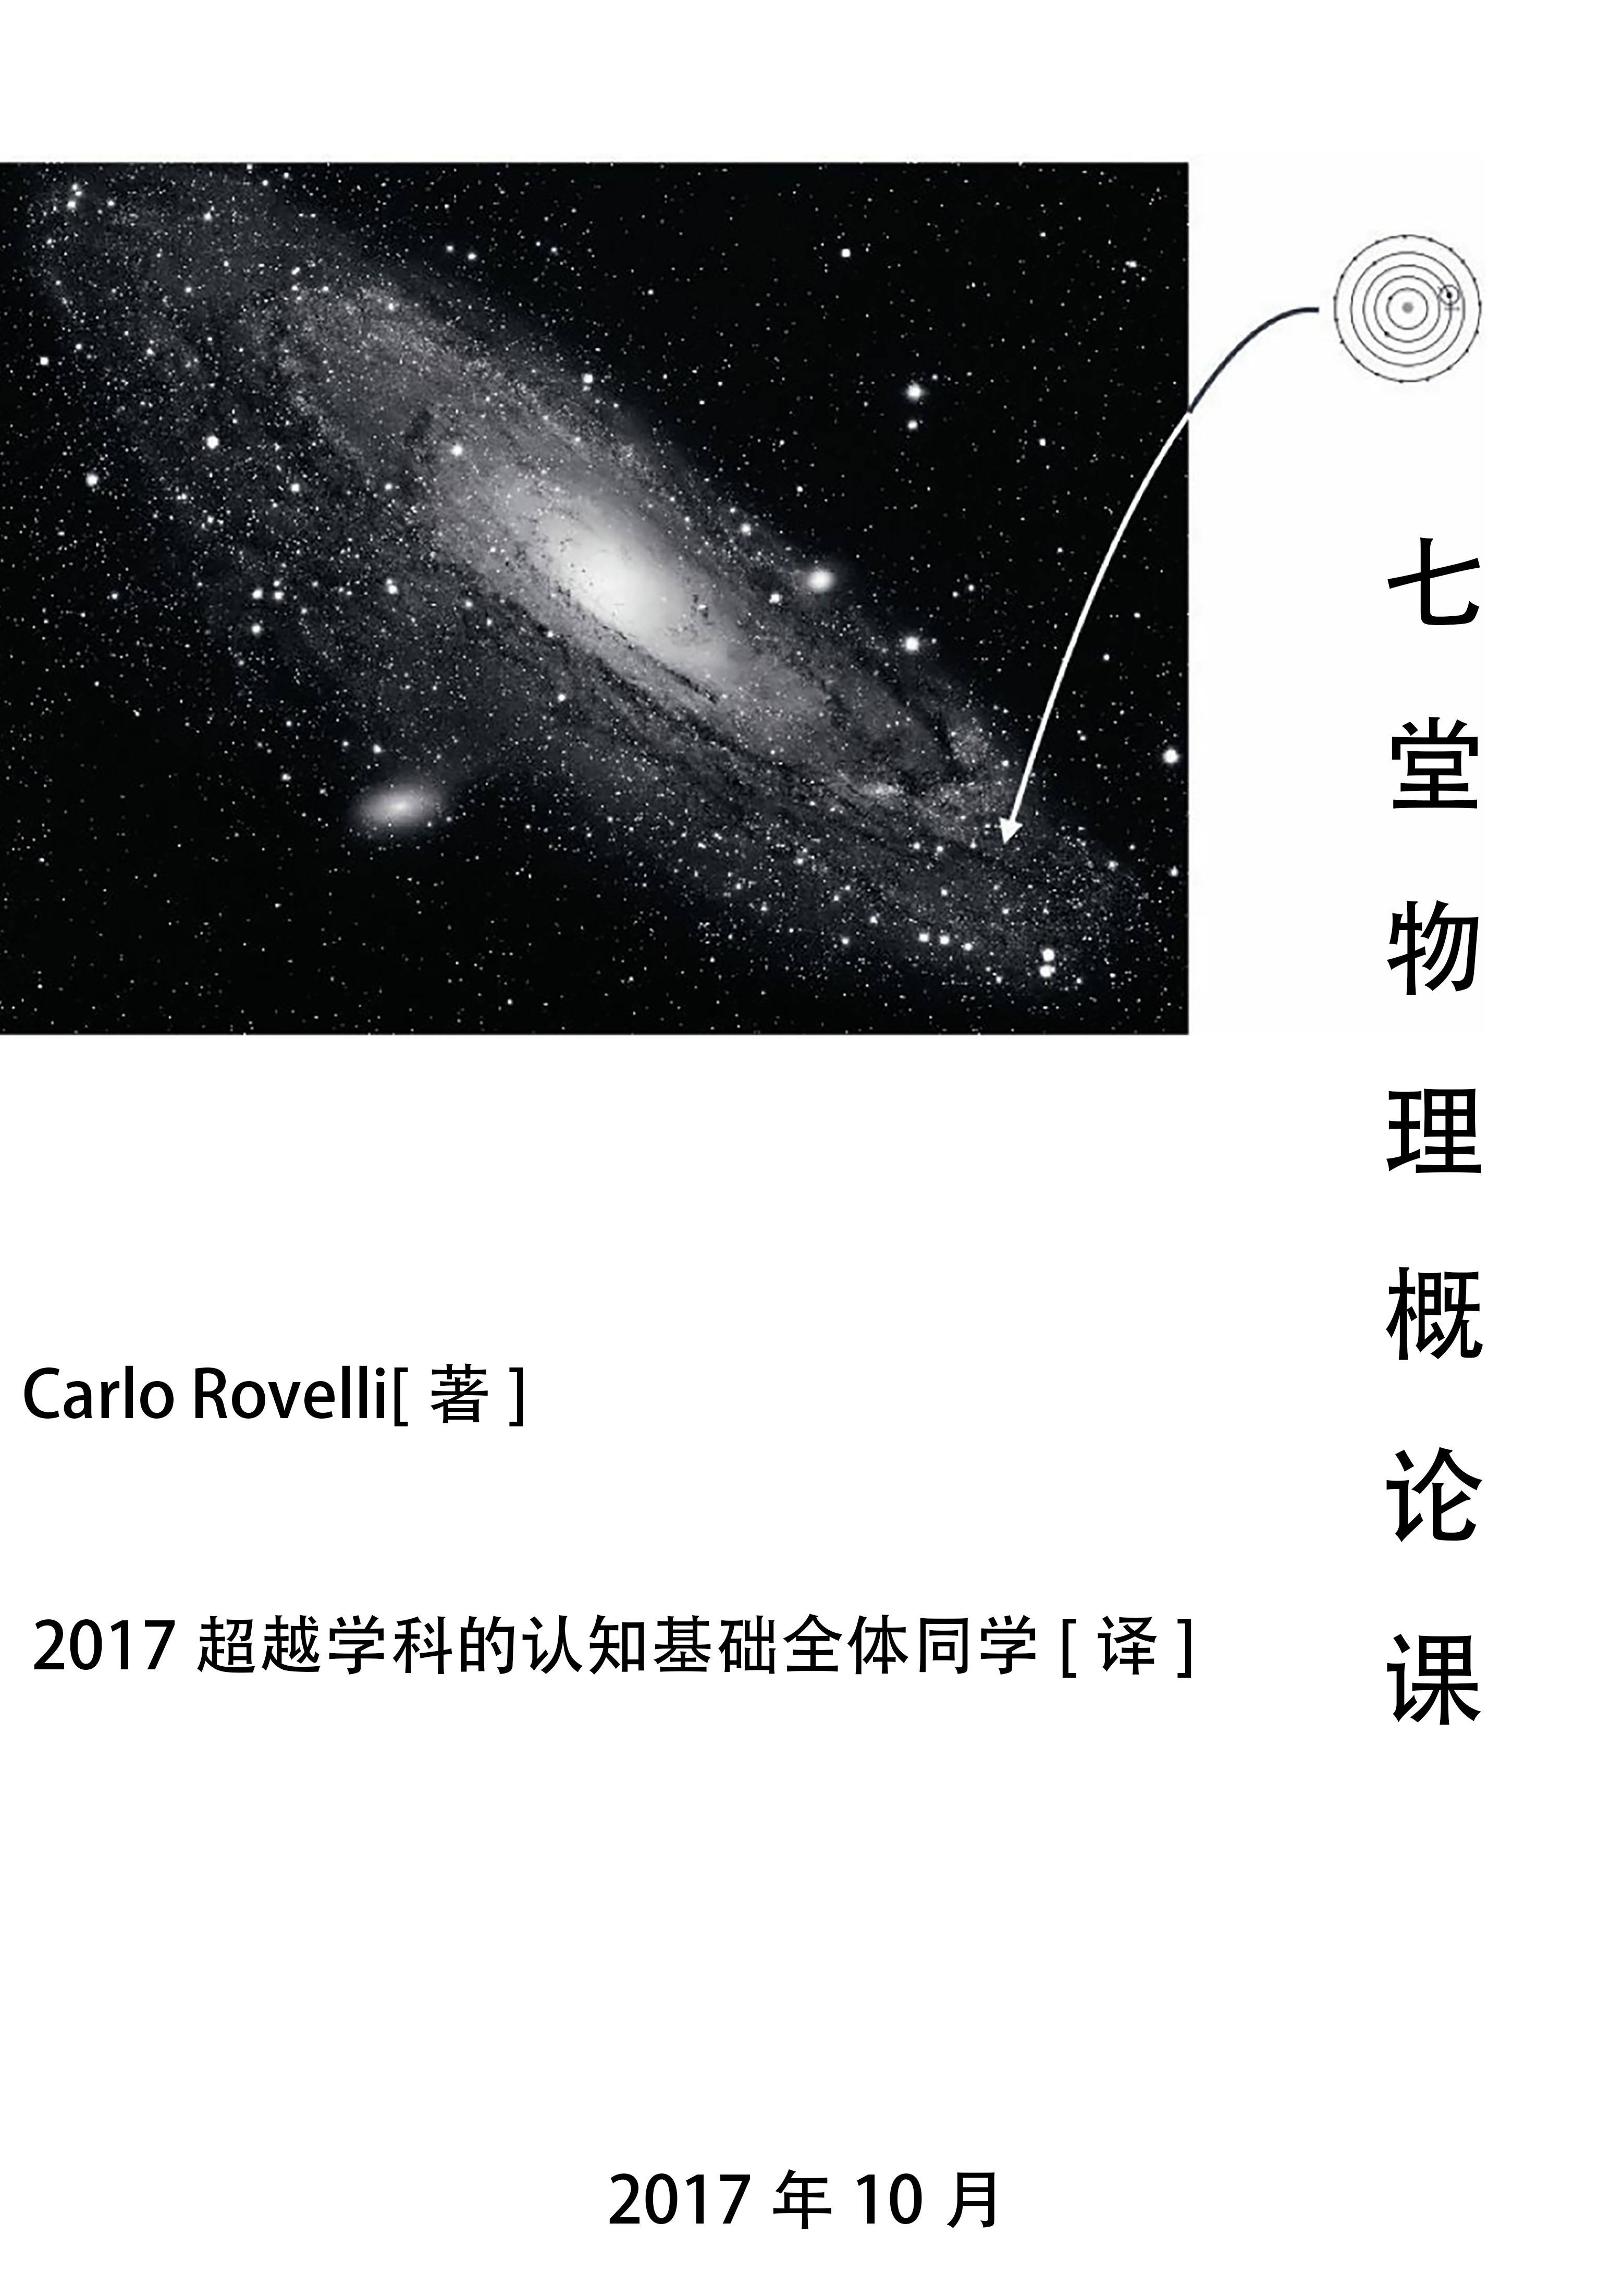
\includegraphics[width=210mm,keepaspectratio]{img/cover.jpg}%
			\vfill
		}%
	}%
}%
\newcommand{\graybox}[3]{%
	\bc\fcolorbox{lightgray}{lightgray!50!white}{%
		\parbox{#1\textwidth}{%
			\bc\parbox{#2\textwidth}{#3}\ec
		}%
	}\ec\par
}
% Fuzz
\hfuzz2pt % Don't bother to report over-full boxes if over-edge is < 2pt
% Listings
\lstset{
	language        = C++,
	breaklines      = true,
	tabsize         = 4,
	frame           = single,
	numbers         = left,
	numberstyle     = \color{gray}\sffamily,
    basicstyle      = \color{violet}\scriptsize\ttfamily,
	keywordstyle    = \color{green!90!black}\bfseries,
	identifierstyle = \color{black},
	commentstyle    = \color{gray}\itshape, % white comments
	stringstyle     = \color{blue},
	showstringspaces= false,
	rulecolor       = \color{lightgray},
	backgroundcolor = \color{lightgray!50!white}
}


\begin{document}

	% Cover and credits -----------------------------------------------------------
	\thispagestyle{empty}
	\pdfbookmark[0]{Cover}{cover}
		\AddToShipoutPicture*{\BackgroundPic}

	\begin{center}

	\end{center}

	\newpage
	\thispagestyle{empty}
	\phantom{hola!}

		
	% Copyright and Credits	
	\null
	\vfill
	\bc
		\begin{minipage}{0.65\textwidth}
			{\sffamily
				\bc
					\textbf{\copyright 2017 \href{http://toyhouse.cc/wiki/index.php/Seven_Brief_Lessons_on_Physics}{\textbf{超越学科界限的认知基础}}}\\
					\textsc{Creative Commons}\\
					Attribution-NonCommercial 4.0 International\\
					\href{http://creativecommons.org/licenses/by-nc/4.0/legalcode}{(CC BY-NC 4.0)}\\[12pt]
					
\includegraphics{img/license.png}\\[12pt]
				\ec
	
				\small\textbf{Cover image:} Little is known about the ultra high-energy cosmic rays that regularly penetrate the atmosphere. Recent IceCube research rules out the leading theory that they come from Gamma Ray Bursts. (Courtesy: NSF/J. Yang).
			}
		\end{minipage}\vspace*{1ex}
		\small\href{http://www.interactions.org/cms/?pid=2100&image_no=DE0106}{\textbf{\url{http://www.interactions.org/cms/?pid=2100&image_no=DE0106}}}
	\ec

	\cleardoublepage

	% Table of contents -----------------------------------------------------------
	%    Title aligned right and in italics
	\titleformat{\chapter}[block]{\raggedleft\itshape}{}
		{0pt}{\parbox{\linewidth}{\raggedleft\vspace*{1em}\Huge#1}}
	\pdfbookmark[0]{Contents}{contents}
	\pagenumbering{roman}           % roman page numbering (invisible for empty page style)

	\pagestyle{plain}               % display just page numbers
	\tableofcontents
	\cleardoublepage
	
		\chapter*{译者序}
	\indent

	

    《七堂极简物理课》是一本由意大利物理学家Carlo Rovelli执笔的广受欢迎的科普读物。
	
	Seven Brief Lessons on Physics is a popular science book written by Carlo Rovelli, an Italian Physicist.

	这本书也被清华大学“超越学科的认知基础”课程所选为编辑wiki的练习对象。其练习目的除了将英文翻译成中文,更重要的是基于译者对文章内容的理解以及他们自己的认知观进行必要的注释。
	
	This book is also used as an exercise for wiki editing for the Cognitive Foundations course at Tsinghua. The purpose is not just to create an English to Chinese translation, but also to annotate the essence of the book based on translators' interpretation.

	



   《七堂极简物理课》是一本很有趣的书

    作者通过对现代物理学许多基本概念的阐述,为读者们构建现代物理学的框架。在保持语言严谨的前提下,又生发以简洁的描述带领读者朋友们走进物理的殿堂。从科学普及的角度来讲,这本书达到了普及物理学的基本要求;从传授知识的角度来讲,虽然许多概念作者并没有给它们以严谨而准确的定义,但是这本书可以成为那些对这些感兴趣的人入门的导引。就像在最美丽的理论那一章所描述的,如果读者对这个问题感兴趣的话,可以自己学习黎曼几何的有关知识,进而对广义相对论的数学要求有一个基本的把握,这之后就可以进行广义相对论的学习。从这个角度来讲本书也达到了传授知识的目的。

    同时,考虑到我们现在这门课的背景,这本书更显得难能可贵——在升华概念的过程中,我们所要学习的不仅仅是概念本身,更多的是人类认识这些概念的过程与方法,这才是认知的核心。而且物理学作为十分艰深的一门学科,有着非常好的代表性与导引性。从这个角度而言,这本书对于我们把我认知的过程,了解认知的细节,都有着十分重要的作用。

                                                                                               ——第一组翻译小组


    《七堂极简物理课》是一本非常值得阅读的书。

    虽然书本身只是由曾刊登在报刊上的七篇小短文组成,但是具有着不一般的价值。首先,这种价值体现在对物理知识的传播上。本书以通俗易懂的语言,向读者介绍了当代最前沿的物理知识,因其使用了大量的比喻等手法,语言生动、讲解深入浅出,作为科普读物广受欢迎。

    其次,这种价值体现在对跨学科认知的启示上。许多跨学科认知的概念都来自物理学,本书内容本身就为跨学科认知的发展提供了良好的语言和知识素材。再者,本书广泛使用本体、空间和系统的隐喻来达到帮助读者跨学科认知的手法十分值得借鉴和学习。可以说,本书一定程度上是一个跨学科认知的成功范例。

    同时,作为“超越学科的认知基础”这门课的同学们的第一个数字流出版物,每名同学都有着很多的付出。从阅读到翻译,再到整理出版,每组成员都有着一定的贡献。如今,这本书的成功出版,令所有人都感到喜悦,同时也坚定了最终制作完全属于自己的数字流出版物的信心。

    不可否认的是,恰恰因为本书语言的简约性,对各个物理概念的说明不够全面、深入。而作为大学生的译者们经验甚浅,难免会有文不达意、粗陋错误之处,还望大家能积极批评指正!

                                                                                               ——第二组翻译小组

    《七堂极简物理课》是一本深入浅出、风趣幽默的科普书。

    本书讲述了近现代的物理学理论的发展,从相对论到量子力学再到整合相对论与量子力学的圈量子引力论等等。提出一个又一个引人深思的问题,又逐一以现有理论进行解答。留给读者思考空间又以现代理论加以阐释,使人很快了解现代物理学的发展方向以及发展近况。

    书中语言风趣幽默,大量使用[[隐喻]]的手法,用人们生活中的常见现象来比喻复杂难懂的物理学概念,易于人们理解接受。同时其又从人物,科技,结构三方面,清晰的给出了物理学的架构。译者认为这不光是一本良好的科普读物,也是应用认知学写作的书籍的良好示范。

    我们的工作在于将本书翻译成了中文,并按照我们的理解添加了很多注释。在翻译文章的同时,我们也在不停的改变着我们对于这世界的认知。本书翻译过程中,融入了多位译者学习到的关于认知学的思想和知识。对于隐喻的理解,以及对于范畴论思想的融汇,使得翻译变得更有认知学思想。这部书不单单是一本物理学的科普书籍。我们更希望向读者呈现出其独特的认知观。

                                                                                               ——第三组翻译小组




	\noindent
	\input{00.abstract.tex}
	\cleardoublepage

	% Document body ---------------------------------------------------------------
	%	 Title over a yellow background
	\titleformat{\chapter}{\normalfont}{}
		{0pt}
		{\begin{tikzpicture}[remember picture,overlay]
			\node[yshift=-7cm] at (current page.north west)
				{\begin{tikzpicture}[remember picture, overlay]
					\draw[fill=yellow,yellow] (0,-1) rectangle
						(\paperwidth,7cm);
					\node[anchor=west,xshift=2\marginparwidth,yshift=2.5cm,rectangle]
						{\fontsize{380}{130}\color{white}\selectfont\AlegreyaBlack\thechapter};
					\node[anchor=west,xshift=5\marginparwidth,yshift=1cm,rectangle]
						{\parbox{\linewidth}{\raggedleft\vspace*{1em}\fontsize{40}{45}\selectfont\AlegreyaBlack#1}};
				 \end{tikzpicture}
				};
		 \end{tikzpicture}
		}
	\titlespacing*{\chapter}{0pt}{100pt}{0pt}

	\pagenumbering{arabic}          % arabic page numbering
	\setcounter{page}{1}            % set page counter
	\pagestyle{maincontentstyle}    % fancy header and footer
		\chapter{最美丽的理论}
\indent

    阿尔伯特·爱因斯坦在年轻的时候有一年都在漫无目的地游手好闲。不幸的是,如果你不“浪费”时间的话,你不会获得任何东西——这一点是青年人的父母常常会遗忘的。他那时在
\href{http://toyhouse.cc/wiki/index.php/帕维亚}{帕维亚}
。他去那里与家人会合,这时的他不得不中断了德国的学业,无法在那里度过充实的高中生活。那时正是二十世纪初,意大利正在工业革命的初级阶段。他的父亲是一名工程师,正在潘丹(paduan)平原建立第一台电力工厂。阿尔伯特那时正在阅读康德的著作,有时还会旁听帕维亚大学的课程:这只是为了开心,而不需要在那里登记或者需要为考试着想。就是在这样的情况下,严肃的科学家才诞生。
\footnote[1]
{
事实上彼时爱因斯坦并没有在德国有一个良好的学习环境,他讨厌那里军国主义的氛围,同时也被老师和同学视为异类,据其自己陈述,:“德国政府过分强调军国主义精神 , 这与我是格格不入的 ,甚至当我还是个孩子的时候就是如此 。我父亲迁居到意大利后 , 在我的请求下 ,他采取措施 ,使我放弃了德国国籍 , 因为我想成为一个瑞士公民 。”《纪念爱因斯坦译文集》 , 赵中立 、许良英编译 , 上海 :上海科学技术出版社 , 1979 年第 1 版 , 第 101~ 102 页 。
}
    
    在登记入学
\href{http://toyhouse.cc/wiki/index.php/苏黎世联邦理工学院}{苏黎世联邦理工学院}
后,他沉浸于物理学的世界中。几年后,1905年,他在当时最为著名的科学杂志,
\href{https://en.wikipedia.org/wiki/Annalen_der_Physik}{Annalen der Physik}
上发表了三篇文章。这三篇文章每一篇都是诺贝尔奖级别的文章。第一篇文章揭示了原子的存在性。第二篇文章为量子力学奠定了最初的基础,我将在下一章详细阐述。第三篇文章提出了他关于
\href{http://toyhouse.cc/wiki/index.php/相对论}{相对论}
最初的理论(今天称之为
\href{http://toyhouse.cc/wiki/index.php/狭义相对论}{狭义相对论}
),这一理论揭示了对于不同的人来说,时间并不是以相同的速度流逝的:如果其中一人以很快的速度移动,那么两个
\href{http://toyhouse.cc/wiki/index.php/孪生子}{孪生子}
会发现他们年龄不同。

    爱因斯坦一夜之间成为了一位著名的物理学家并得到了许多高校的聘书。但是还是有一些事情使他烦躁:尽管这一理论产生了轰动效应,但它并没有与我们所知的引力发生联系,即物理下落的原因。当他为他的理论写一篇总结时,他意识到这一点,并开始思考由现代物理学之父牛顿所提出的引力公式是否需要修改,以使其与新的相对性观念相吻合。他埋头于这一问题中,他花了十年时间去解决这一问题。这十年时间充满了枯燥的学习,尝试,错误,混乱,错误的文章,新奇的想法和被误解的观点。最终,在1915年的11月,他呈递了一份彻底解决这一问题的文章:一个关于引力的新理论,他称之为
\href{http://toyhouse.cc/wiki/index.php/广义相对论}{广义相对论}
——这是他的杰作,被伟大的俄罗斯物理学家
\href{https://en.wikipedia.org/wiki/Lev_Davidovich_Landau}{列夫·朗道}称为“最美丽的理论”。
\footnote[2]
{
从某种程度来讲,狭义相对论是为了解决电动力学的非自洽问题,而广义相对论是为了解决引力问题。
}

    有很多的杰作使我们十分感动:\href{https://en.wikipedia.org/wiki/Wolfgang_Amadeus_Mozart}{莫扎特}的
\href{http://toyhouse.cc/wiki/index.php/安魂曲}{安魂曲};荷马的\href{http://toyhouse.cc/wiki/index.php/奥德赛}{奥德赛};\href{http://toyhouse.cc/wiki/index.php/西斯廷教堂}{西斯廷教堂};\href{http://toyhouse.cc/wiki/index.php/李尔王}{李尔王}。去完全欣赏它们的优美之处往往需要很长的学徒期,但是这种奖赏是纯粹的美丽——但是又不止于此,这一理论使我们有了一种崭新的审视世界的视角。爱因斯坦的宝石,广义相对论,是描述自然界秩序的杰作。

    我还记得我开始理解广义相对论的兴奋与激动。那是一个夏天,我正在卡拉布里亚的Condofuri的海滩上,沐浴在希腊地区地中海的阳光下,还有一年就要大学毕业。一个人只有在不被上学分心的时候,才能最佳地学习。我那时正在一本被老鼠咬破边缘的书的帮助下学习,这是因为在晚上我用这本书来堵住一个位于Umbrian山丘上的破旧房子的老鼠洞,从前我常常在这间房子里来逃避一些无聊的大学课程。我总是会从书中抬起头看远方波光粼粼的大海:我好像真正看见了爱因斯坦所想象的空间和时间的弯曲。这一切好像是魔法:好像是一个朋友在低声告诉我一个非凡的秘密,突然间揭开了现实的面纱,使之显露出一个更为简单也更为深刻的秩序。自从我们发现地球是圆的并且像一个陀螺一样不断自转,我们就已经发现现实并不是看上去那样:每次我们发现现实的一个新方面的知识,我们就会感受到一次深刻的情感体验。又一层面纱被我们撕掉了。

    但是在历史上超越我们的认知的一个接着一个的发现中,爱因斯坦或许是无可匹敌的。这是为什么呢?

    首先,一旦你理解了相对论,你就会发现它那优美的简洁性。我会总结这一观点。

    牛顿尽最大努力去解释物体要掉落和行星要公转的原因。他设想了一个使得所有物体聚集在一起的力,称之为\href{http://toyhouse.cc/wiki/index.php/引力}{引力}。这个力在距离很远但是中间没有其它物体的物体之间发生作用的途径还是未知的——而且牛顿很谨慎地给出了一个假设。他想象物体在空间中移动,空间本身像一个非常大的空容器,大到将整个宇宙都囊括进入,在这个容器中的所有物体都各行其是,直到有力使它们的轨迹发生弯曲。这个牛顿发明的包括整个世界的容器——空间是由什么组成的,他自己也说不清楚。但是爱因斯坦出生后几年,两位伟大的英国物理学家\href{https://en.wikipedia.org/wiki/Michael Faraday}{迈克尔·法拉第}和\href{https://en.wikipedia.org/wiki/James Clerk Maxwell}{詹姆斯·麦克斯韦}向牛顿的经典力学体系中添加了关键性的一部分:那就是\href{http://toyhouse.cc/wiki/index.php/电磁场}{电磁场}。这个场是一个真实的实体,充斥空间,传播\href{http://toyhouse.cc/wiki/index.php/电磁波}{电磁波},可以像湖面一样\href{http://toyhouse.cc/wiki/index.php/振动}{振动},借此传递\href{http://toyhouse.cc/wiki/index.php/电磁力}{电磁力}。由于爱因斯坦年轻的时候就被驱动他父亲所建立的发电厂中转子运动的电磁场所吸引,他不久后就理解了引力,像电场力一样,一定是被一个场所传播的:一个类比于电磁场的\href{http://toyhouse.cc/wiki/index.php/引力场}{引力场}一定是存在的。他的目标是理解引力场的工作规律,以及用数学方程式描述它。

    在那时他想到了一个非凡的想法,一个完全是天才的想法:引力场并不是充斥于空间的,引力场就是空间本身。这就是广义相对论的雏形。牛顿的空间,就是物体移动所有经过的空间,以及引力场是完全相同的一个事物。

    这是一个富有启迪的时刻。一个对于世界极为重要的简化:空间不再是和物质无关的事物,它也是一种组成这个世界的物质。它是一个可以弯曲的事物。我们并不是被装在一个僵硬的看不见的结构中:我们处于一个非常大的弹性蜗牛壳中。太阳使得它周围的空间弯曲,而地球也不是因为一种神秘的力才绕着太阳公转,它是因为它向太阳笔直前进,像一块大理石在漏斗表面滚动一样。在漏斗中央并不存在一个维持这一切的神秘的作用力;是被弯曲的空间导致了大理石的滚动。行星的绕日公转,以及物体的下落,都是因为空间被弯曲了。
\footnote[3]
{
作者在这里描述得十分简单,但简单的原理背后蕴含着复杂的数学推演与逻辑判断,这需要高深的数学和物理学知识,如果读者希望能深入了解这一部分内容,建议优先学习黎曼几何等数学知识,打好基础后再对广义相对论作进一步研究,以避免直接接触高深的物理学知识而无所适从。
}

    我们怎样才能描述空间的曲率呢?十九世纪最为杰出的数学家,有“数学王子”之称的\href{https://en.wikipedia.org/wiki/JJohann Carl Friedrich Gauss}{卡尔·弗里德里希·高斯},已经提出了描述二维曲面,例如山丘表面,的数学方程式。之后,他让一个聪明的学生去将这一理论推广至三维乃至更多维空间中。回答这一问题的学生,\href{https://en.wikipedia.org/wiki/Georg Friedrich Bernhard Riemann}{伯纳德·黎曼},提出了一种对这一问题影响深远的基本原则,尽管看上去它完全是无用的。黎曼论述的结论是弯曲空间是被特定数学实体承载,这一数学实体我们今天称之为\href{http://toyhouse.cc/wiki/index.php/黎曼曲面}{黎曼曲面},通常用R来标记。爱因斯坦提出了一个方程式,在这一方程式中R等价于物体的能量。这就是说空间在有物质存在的地方会发生弯曲。结论就是这样。(The equation fits into half a line, and there is nothing more)如果说这一等式解决了一半的问题,那么这里就没有其它的问题了。一个空间弯曲的观测结果变成了一个等式。
\footnote[4]
{
事实上高斯已经提出了计算空间曲率的一般方法,只是没有完全搭建起来后面我们所称的黎曼几何的数学体系。
}


    但是,这一个方程式描述了整个宇宙。这一理论的丰富性在这里打开一连串幻觉似的的预言,这些预言像极了疯子的的胡言乱语,但是这些在之后都被证明是真的。
 
   首先,这一方程式描述了星体周围的空间是怎样弯曲的。因为曲率的存在,不仅仅行星绕着恒星公转,而且光线也不再沿着直线传播而是发生一定的偏转。在1919年,这一偏转被测量了出来,结果和理论符合的很好。但不仅仅空间会弯曲,时间也会弯曲。爱因斯坦预言在地球表面,相较于低处而言,在高处时间会流逝地更快。这也被实验所证实了。如果一个住在海平面高度的人和他住在山上的孪生兄弟相遇,他会发现他兄弟会比他稍稍老一点。而这才是刚刚开始。

    当一个大的星体烧尽了它所有的可燃烧的物质(氢)时,它就会坍塌。当剩余的部分不再能承载燃烧的热时,它就会由于自身的重量坍塌,直到它使得空间坍塌到产生一个真实的洞。这就是著名的\href{http://toyhouse.cc/wiki/index.php/黑洞}{黑洞}。当我在大学学习这些时,它们仅仅被认为是这一复杂理论的可能预言。今天,他们被数以百计地观测出来,并被天文学家们仔细地研究。

    但这依旧不是全部内容。这个空间都可以膨胀或者收缩。而且,爱因斯坦的方程式揭示了空间不可能是静态的,它一定是在膨胀。在1930年,宇宙的膨胀被真正地观测出来。同样的一个方程预言这一膨胀应该是被一个年轻的非常小但非常热的宇宙爆发所引起的:现在我们称之为“\href{https://en.wikipedia.org/wiki/Big Bang}{大爆炸理论}”。又一次,最初没有人相信这一理论,但是相关的证据一直积累到\href{http://toyhouse.cc/wiki/index.php/宇宙背景辐射}{宇宙背景辐射}——由于最初爆炸所产生扩散的微波——被直接观测到。爱因斯坦方程式所产生的预言又一次被证明是正确的。但是进一步,这一理论断言空间像大海的表面一样运动。这些引力波的影响在宇宙中的双星系统中被观测出来,又一次与这一理论的预言相吻合,甚至吻合到令人惊讶的一千亿分之一的数量级上。其它情况也是这样。
\footnote[5]
{
作者没有提到,这一千亿分之一事实上也是物理学关注的一个焦点:如果只有所有参数都恰到好处才会产生我们这样的宇宙,那是否说明我们这样的宇宙有些过于特殊了呢?
}

    简而言之,这一理论描述了一个多姿多彩并且令人惊奇的世界。在这里,宇宙爆炸,空间坍塌成为一个无底洞,时间在行星附近变得缓慢,无边无际的星际空间像大海表面一样波动……这所有的一切,都渐渐地在我那本被老鼠咬过的书中出现,但它们并不是一个精神错乱的白痴所讲的故事,也不是一个被卡拉比亚地区地中海的烈日和令人眩晕的大海所引发的幻觉。这一切都是现实。

    或者更好地说,现实的一小部分,只是现实所蒙上诸多面纱中的一小部分。这个现实似乎是由和构成我们梦境相同的事物所构成的,但是比我们朦胧的梦境更为真实。

    所有的这一切都是一个基本的直觉的结果:空间和引力场是同样的一个东西。尽管你们几乎一定不能去理解这一简单的方程式,但我还是要在这里写下它。或许任何读到这的人都能去欣赏它那完美的简洁性:
    
$$R_{ab}-\frac{1}{2}Rg_{ab}=T_{ab}$$                      

    就是这样。

    你或许,当然,为了掌握阅读和使用这一方程式需要去学习和理解黎曼的数学工具。这会耗费一些时间和精力。但是相对于欣赏贝多芬后期弦乐曲秘密的美丽,这都是次要的。在这两种情形下,奖赏都是纯粹的美丽,以及看待世界的一种崭新视角。



\noindent
\iffalse
	\graybox{.8}{.65}{
		\bc\textcolor{gray}{\Large{\sffamily Notation used in this document:}}\ec

		\textbf{Abbreviations:}

		EM: electro-magnetic,\\
		UV: ultra-violet,\\
		$\gamma$: gamma-rays,\\
		X: X-rays,\\
		$e^-$: electron,\\
		$\pi$: pion,\\
		$\mu$: muon,\\
		$\nu$: neutrino, etc.\vspace{2ex}

		\textbf{Units:}\\
		International System:\\
		eV: electron volts,\\
		J: Joules,\\
		C: Celsius,\\
		M: mega,\\
		G: giga, etc.\vspace{2ex}

		\textbf{Chemical symbols:}\\
		The elements of the periodic table.\vspace{2ex}

		\textbf{References:}\\
		There are internal (marked in \textcolor{red}{red}) and external (marked in \textcolor{blue}{blue}) references.\vspace{2ex}
	}
\fi

		\chapter{量子}
\indent

我可以很确定的告诉大家:没有人真正了解量子力学。——狄拉克

一个物理学系统——原子的任何一种结合体——什么时候才显示出“动力学的定律”(在普朗克的意义上说)或“钟表式工作的特点”呢?量子论对这个问题有一个简短的回答,就是说,

在绝对零度时。当接近零度时,分子的无序对物理学事件不再有什么影响了。这是沃尔塞.能斯特的著名的“热定理”,有时候被冠以“热力学第三定律”的美名(第一定律是能量原理,第二定律是熵原理)。——《生命是什么》


    二十世纪物理学的两大支柱——我在第一章所提到的
\href{http://toyhouse.cc/wiki/index.php/广义相对论}{广义相对论}和现在我将要阐述的[[量子力学]],不同到不能再不同了。这两个理论都告诉我们精致的自然结构事实上比看上去更为细小。但是广义相对论是一个杰出的佳作:作为由[[爱因斯坦]]独立思考到的成果,它是一个将引力场,空间和时间视为简单的连续体来处理的。而量子力学或“量子理论”,在另一方面,其得到了无比成功的实验验证并且已经产生了一些改变我们每日生活的产品(例如,我正在使用的电脑)。然而在它诞生一个多世纪后,它还是十分神秘并且难以理解。
    据说量子力学准确地诞生于1900年,之后引导了一个世纪的诸多艰深的思考。德国物理学家
\href{https://en.wikipedia.org/wiki/马克思·普朗克}{Max Planck}计算了黑体内的辐射场。为了计算,他用了一个巧妙的方法:他想象场的能量被分配在量子中,就是说能量被分为一块一块的。这一过程计算出了和实验符合的非常好的结果(因此,在一定程度上是正确的)但是却和当时所知的所有物理规律相违背。能量一直以来被认为是连续变化的,并且没有理由去把它处理成由小的结构单元组成。对普朗克本人来说,把能量处理成由有限的结构单元组成也是一种奇怪的计算方法,他自己也没有完全理解这种方法的有效性。再一次,是五年后爱因斯坦理解了能量单元是真实存在的。爱因斯坦认为光是由能量单元组成的——光单元。今天我们称它们为[[光子]]。他在他文章的介绍中写道:''我认为,如果我们假设光的能量是不连续分布在空间中,那么与[[黑体辐射]],[[荧光]],由[[紫外光]]激发的[[阴极射线]]以及其它与光产生与传播相关的物理现象都能够更好地被理解。与假设保持一致,点光源发射的光的能量在扩张的空间中是不连续分布的,而且是由有限个位于空间中某个点的能量量子组成的,他们在移动中不会被拆分,只能作为整体产生或被吸收。''
\marginpar{*译者注1:作者在这里的描述似乎不够准确,前人在计算的时候将能量设想为一块一块的,普朗克本人并没有创造这种方法,但具有革命性意义的是,前人在计算的时候认为一块一块的能量每一块最后都是趋近于0的,但普朗克认为每一块都是一个非常小的常数,并不是0。}


    这一段简洁而清晰的论断才是量子理论诞生的标志。注意到开始的“我认为”,使我想起了“我认为……”,就像达尔文介绍进化论时,或者法拉第第一次介绍关于磁场的革命性的理论时所说的。天才也是会犹豫的。
    爱因斯坦的工作最初被物理学界的同仁认为是一个杰出年轻物理学家无意义的幼稚之作。但是随后,正是因为这项工作他被授予了诺贝尔奖。如果说普朗克是量子理论之父的话,那么爱因斯坦则是养育它的人。
{{注释|注释=
*译者注2:虽然爱因斯坦获得过诺贝尔奖这件事情广为人知,但是爱因斯坦获奖原因是光电效应领域的开创性的研究,而不是像很多人所想的那样是由于狭义相对论和广义相对论的突出贡献。因为彼时相对论并没有被物理学界完全接受。
}}
    但是就像所有的后代一样,这一理论之后在爱因斯坦没有预料到的情况下自行发展。在二十世纪第二个和第三个十年,[[wikipedia:Niels Bohr|戴维·尼尔斯·玻尔]]领导了量子理论的发展。玻尔理解了原子中电子的能量只能取固定的几个值,就像光的能量一样。重要的是,电子只能在能量一定的[[原子轨道]]之间[[跃迁]],发射或吸收一个光子。这就是著名的[[量子跃迁]]。除此之外,在他位于哥本哈根的研究院内聚集了那个世纪最为杰出的青年物理学家,他们一起探索并且试图将原子世界一些令人困惑的现象澄清,最终建立一个连贯的理论。在1925年,这一理论的基本方程出现了,代替了全部的[[牛顿力学]]。
    很难想象比这更为杰出的成就了。一时间,所有事情都有意义了,你也可以计算所有的事情。例如:你是否还记得[[wikipedia:Dmitri Mendeleev|门捷列夫]]所发明的被挂在很多教室的墙上,囊括了所有宇宙中的元素,从[[氢]]到[[铀]]的元素周期表吗?为什么每个元素都被放在了特定的位置?为什么元素周期表有其特定的结构、周期?又为什么元素有这样那样的特性呢?答案就是每个元素对应着量子力学主方程式的一个特解。整个化学都由一个方程式衍生而来。
    第一个依据那些令人眼花缭乱的假设写下这个方程的人,是德国的天才青年物理学家[[wikipedia:沃纳·海森堡|沃纳·海森堡]]。
{{注释|注释=
*译者注3:海森堡率先创建了矩阵力学,随后薛定谔创建了波动力学并且证明了它们二者的等价性。我们目前所写的基本方程,大多是薛定谔方程。
}}
    海森堡认为电子并不总是存在的。它们只在有人或者仪器观察它们的时候,或者更准确地说,它们和其它事物发生相互作用的时候才存在。它们当与其它事物碰撞的时候,会在空间中以一定可计算的概率具象化。由一个轨道到另一个轨道量子跃迁是它们具象化的唯一方法:一个电子是一系列由一次相互作用到另一次相互作用的跃迁,电子并不位于任何准确的位置。它根本不在空间中。
    这就好像上帝并没有用一个加粗的线来设计现实,只是用点来描述它的轮廓。
    在量子力学中,不存在具有准确位置的物体,除了当它们飞快地和其它事物碰撞时。为了描述由一次相互作用到另一次相互作用的碰撞期间的物理过程,我们用一种不存在于真实物理空间,仅仅存在于抽象数学空间的抽象数学模型来刻画这一过程。但是更糟糕的事情发生了:这些相互作用的跃迁并不是以可预测的方式发生,而是很大程度上随机发生。我们不可能去预言电子将会在哪里重新出现,而只能去计算它会在这里或那里出现的[[概率]]。关于概率的问题深深困惑着那些认为所有事情都是由坚固、普遍并且不可动摇的物理学规律控制的物理学家们。   
    这听上去荒唐吗?这对爱因斯坦也十分荒唐。一方面,他提名海森堡获诺贝尔奖,因为意识到他理解了一些关于这世界基础的规律;另一方面,他不放过任何机会去抱怨这理论毫无意义。
    [[wikipedia:Niels Bohr Institute|哥本哈根学派]]的年轻学者们十分沮丧:爱因斯坦怎么像这样来想?他们的精神领袖,那个曾经有勇气去思考不能思考的事物的大师,现在退缩了,畏惧这他自己所引发的到未知领域的跳跃。那个认为时间并不是永恒不变的和空间是卷曲的爱因斯坦现在却认为世界并不可能这样奇异。
    玻尔耐心地把这些新理论解释给爱因斯坦。爱因斯坦否认了这一理论。他设计了思想实验去证明这一新理论是自相矛盾的:“想象一个充满光的盒子,从这里我们允许单个的光子消失一瞬间……”之后就是他最著名的例子之一,“光盒(box of light)实验。最终波尔总能找到驳斥这些否认的答案。他们之间的对话以讲座,书信以及论文等等方式持续了很多年。在交换观点的过程中,这两位伟人都需要重新思考以调整他们的光点。爱因斯坦不得不承认新理论中不存在矛盾之处。玻尔不得不承认事情并不是像他一开始想的那样简单与清晰。爱因斯坦不想在总是存在一个不依赖于相互作用而存在的客观真实这一观点上让步。同样地,玻尔也不想在建构现实的新理论的可信性上让步。最终,爱因斯坦承认量子论是一个理解世界方面巨大的进步,但仍认为事物不应该像假设一样奇怪——这理论的背后一定存在一个更为深刻和理性的解释。
    一个世纪以后,我们现在面临着相同的问题。量子力学的方程及其解被物理学家,工程学家,化学家和生命科学家广泛地应用在不同的领域。它们在所有当代技术的领域都十分有用。但它们还是十分神秘。因为它们并没有描述物理系统内究竟发生了什么,只是刻画了一个物理系统是如何影响另一个物理系统的过程。
{{注释|注释=
*译者注4:非常著名的一个思想实验是薛定谔提出的“薛定谔的猫”实验。在这一实验中,尽管我们可以描述量子的不确定态,但是与宏观物体建立联系后,宏观物体似乎也处于一种“死生叠加态”。这一问题至今没有得到合理的解释。
}}
    这意味着什么?一个系统重要的真实性是不可描述的吗?这是否意味着我们只是缺少一部分谜题?或者这是否意味着,至少对我来说,我们必须接受现实仅仅是相互作用?我们在现实领域的知识总量在不断增加,这使得我们可以做一些我们过去甚至难以想象的事情。但是这增加又提出了新的问题,新的神秘。那些在实验室使用这些理论的人继续探索不管这些问题,但是在近些年数量急剧增加的文章和会议中,物理学家和哲学家继续去研究这些问题。在它诞生一个世纪以后,什么是量子理论?是一个对于自然真实性非常深刻的尝试?还是一个巧合与事实相符的大错?或是一个不完全谜题的一部分?亦或是一个深刻的关于世界结构的但我们目前还无法理解的理论的线索?
    爱因斯坦去世后,他最伟大的对手玻尔向他致以崇敬欣赏的悼词。当几年后玻尔去世时,有人拿出了他研究过程中的一块黑板的照片。在黑板上有一幅画。画所描述的是爱因斯坦思想实验中的“充满光的箱”。到最后,还是渴望去挑战自己以获得更多的认识与理解。到最后,还是对于事物本质的怀疑。
{{注释结束}}
    二十世纪物理学的两大支柱——我在第一章所提到的广义相对论和现在我将要阐述的量子力学,不同到不能再不同了。这两个理论都告诉我们良好的自然结构比看上去更为细小。但是广义相对论是一个紧凑的佳作:作为由爱因斯坦自己思考到的成果,它是一个对于引力,空间和时间简单并且连贯的观点。而量子力学或“量子理论”,在另一方面,已经得到不相匹配的实验成功并且已经产生了改变我们每日生活的产品(例如,我正在使用的电脑)。但是在它诞生一个多世纪后,它还是十分神秘并且难以理解。

  据说量子力学是准确地在1900年诞生,几乎引导了一个世纪的很多思考。德国物理学家马克思.普朗克计算了黑体内的辐射场。为了计算,他用了一个巧妙的方法:他想象场的能量被分配在量子中,就是说能量被分为一块一块的。这一过程导致了和实验符合非常好的结果(因此,在一定程度上是正确的)但是却和当时所知的所有物理规律相违背。能量一直以来被认为是连续变化的,并且没有理由去把它处理成由小的结构单元组成。对普朗克本人来说,把能量处理成由有限的结构单元组成也是一种奇怪的计算方法,他自己也没有完全理解这种方法的有效性。再一次,是五年后爱因斯坦理解了能量单元是真实的。爱因斯坦认为光是由能量单元组成的——光单元。今天我们称它们为光子。他在他的文章的介绍中写道:我认为,如果我们假设光的能量是不连续分布在空间中,那么与黑体辐射,荧光,由紫外光激发的阴极射线以及其它与光产生与传播相关的物理现象都能够更好地被理解。与假设保持一致,点光源发射的光的能量在扩张的空间中是不连续分布的的,而且是由有限个位于空间中某个点的能量量子组成的,他们在移动中不会被拆分,只能作为整体产生或被吸收。

  这一段简洁而清晰的论断才是量子理论诞生的标志。注意到开始的“我认为”,使我想起了“我认为……”,就像达尔文介绍进化论时,或者法拉第第一次介绍关于磁场的革命性的理论时所说的。天才也是会犹豫的。

  爱因斯坦的工作最初被物理学界的同仁认为是一个杰出年轻物理学家无意义的幼稚之作。但是随后,因为同样的工作他被授予了诺贝尔奖。如果说普朗克是量子理论之父的话,那么爱因斯坦则是养育它的人。

  但是就像所有的后代一样,这一理论之后在爱因斯坦没有预料到的情况下自行发展。在二十世纪第二个和第三个十年,戴维·尼尔斯·玻尔领导了量子理论的发展。波尔理解了原子中电子的能量只能取固定的几个值,就像光的能量一样。重要的是,电子只能在能量一定的原子轨道之间跃迁,发射或吸收一个光子。这就是著名的量子跃迁。除此之外,在他位于哥本哈根的研究院内聚集了那个世纪最为杰出的青年物理学家,他们一起探索并且试图将原子世界一些令人困惑的现象澄清,最终建立一个连贯的理论。在1925年,这一理论的基本方程出现了,代替了全部的牛顿力学。

  很难想象比这更为杰出的成就了。一时间,所有事情都有意义了,你也可以计算所有的事情。例如:你是否还记得门捷列夫所发明的有这些周期和有这些特定性质的元素的结构?答案就是每个元素对应着量子力学主方程式的一个特解。化学由一个方程式产生。

  第一个依据那些令人眼花缭乱的假设写下这个方程的人,是德国的天才青年物理学家沃纳·海森堡。元素周期表,那上面列出了由氢到铀组成宇宙的所有可能的元素,因此被挂在很多教室的墙上。为什么就是这些元素被列举在这里以及为什么元素周期表

  海森堡认为电子并不总是存在的。它们只在有人或者仪器观察它们的时候,或者更准确地说,它们和其它事物发生相互作用的时候才存在。它们当与其它事物碰撞的时候,会在空间中以一定可计算的概率具象化。由一个轨道到另一个轨道量子跃迁是它们具象化的唯一方法:一个电子是一系列由一次相互作用到另一次相互作用的跃迁,电子并不位于任何准确的位置。它根本不在空间中。

  这就好像上帝并没有用一个加粗的线来设计现实,只是用点来描述它的轮廓。

  在量子力学中,不存在具有准确位置的物体,除了当它们飞快地和其它事物碰撞时。为了描述由一次相互作用到另一次相互作用的碰撞期间的物理过程,我们用一种不存在于真实物理空间,仅仅存在于抽象数学空间的抽象数学模型来刻画这一过程。但是更糟糕的事情发生了:这些相互作用的跃迁并不是以可预测的方式发生,而是很大程度上随机发生。我们不可能去预言电子将会在哪里重新出现,而只能去计算它会在这里或那里出现的概率。关于概率的问题深深困惑着那些认为所有事情都是由坚固、普遍并且不可动摇的物理学规律控制的物理学家们。   

   这听上去荒唐吗?这对爱因斯坦也十分荒唐。一方面,他提名海森堡获诺贝尔奖,因为意识到他理解了一些关于这世界基础的规律;另一方面,他不放过任何机会去抱怨这理论毫无意义。

   哥本哈根学派的年轻学者们十分沮丧:爱因斯坦怎么像这样来想?他们的精神领袖,那个曾经有勇气去思考不能思考的事物的大师,现在退缩了,畏惧这他自己所引发的到未知领域的跳跃。那个认为时间并不是永恒不变的和空间是卷曲的爱因斯坦现在却认为世界并不可能这样奇异。

  玻尔耐心地把这些新理论解释给爱因斯坦。爱因斯坦否认了这一理论。他设计了思想实验去证明这一新理论是自相矛盾的:“想象一个充满光的盒子,从这里我们允许单个的光子消失一瞬间……”之后就是他最著名的例子之一,“光盒(box of light)实验。最终波尔总能找到驳斥这些否认的答案。他们之间的对话以讲座,书信以及论文等等方式持续了很多年。在交换观点的过程中,这两位伟人都需要重新思考以调整他们的光点。爱因斯坦不得不承认新理论中不存在矛盾之处。玻尔不得不承认事情并不是像他一开始想的那样简单与清晰。爱因斯坦不想在总是存在一个不依赖于相互作用而存在的客观真实这一观点上让步。同样地,玻尔也不想在建构现实的新理论的可信性上让步。最终,爱因斯坦承认量子论是一个理解世界方面巨大的进步,但仍认为事物不应该像假设一样奇怪——这理论的背后一定存在一个更为深刻和理性的解释。

  一个世纪以后,我们现在面临着相同的问题。量子力学的方程及其解被物理学家,工程学家,化学家和生命科学家广泛地应用在不同的领域。它们在所有当代技术的领域都十分有用。但它们还是十分神秘。因为它们并没有描述物理系统内究竟发生了什么,只是刻画了一个物理系统是如何影响另一个物理系统的过程。

  这意味着什么?一个系统重要的真实性是不可描述的吗?这是否意味着我们只是缺少一部分谜题?或者这是否意味着,至少对我来说,我们必须接受现实仅仅是相互作用?我们在现实领域的知识总量在不断增加,这使得我们可以做一些我们过去甚至难以想象的事情。但是这增加又提出了新的问题,新的神秘。那些在实验室使用这些理论的人继续探索不管这些问题,但是在近些年数量急剧增加的文章和会议中,物理学家和哲学家继续去研究这些问题。在它诞生一个世纪以后,什么是量子理论?是一个对于自然真实性非常深刻的尝试?还是一个巧合与事实相符的大错?或是一个不完全谜题的一部分?亦或是一个深刻的关于世界结构的但我们目前还无法理解的理论的线索?

  爱因斯坦去世后,他最伟大的对手玻尔向他致以崇敬欣赏的悼词。当几年后玻尔去世时,有人拿出了他研究过程中的一块黑板的照片。在黑板上有一幅画。画所描述的是爱因斯坦思想实验中的“充满光的箱”。到最后,还是渴望去挑战自己以获得更多的认识与理解。到最后,还是对于事物本质的怀疑。

\noindent

		\chapter{宇宙的结构}
\indent

    在20世纪前半页,
\href{http://toyhouse.cc/wiki/index.php/爱因斯坦}{爱因斯坦}
(Einstein)描述了时间与空间的原理,与此同时,
\href{http://toyhouse.cc/wiki/index.php/尼尔斯·玻尔}{尼尔斯·玻尔}
(Niels Bohr)和他年轻的学徒醉心于研究描述物质奇异
\href{http://toyhouse.cc/wiki/index.php/量子}{量子}
现象的方程。在这一世纪的下半叶,物理学家们在这两个理论基础之上,把这两个全新的理论应用到描述自然现象的各个领域:从宇宙的宏观结构到
\href{http://toyhouse.cc/wiki/index.php/基本粒子}{基本粒子}
的微观结构。我将在这一章讲述前者,在下一章讲述后者。


    这一章的组成大部分都是简笔画。这样做的原因是,在实验,测量,数学以及严密的推理之前,科学是建立在关于视野的一切之上的。科学从视野开始。科学的思维是被从同以往不同的角度“看待”事物的能力培养出的。在不同视野间遨游,而我想在此提供这次物理学之行的简要适度的轮廓。
\footnote[1]
{
科学建立在视野之上,在这里视野指的某种可观测的对象。后面的例子以宇宙作为观测对象;而前面提到的两个科学家的视野则分别是,爱因斯坦看到的
\href{http://toyhouse.cc/wiki/index.php/电磁学}{电磁学}
中光速不变,以及玻尔看到的原子分立光谱。
}

\begin{figure}[htbp]
\begin{minipage}[t]{0.3\linewidth}
\centering
\bc
\includegraphics[width=3\textwidth]{img/31.jpg}\\[12pt]
\ec
\caption{这幅图上下的概念在原文中已经有所展示了,但是并非所有的早期宇宙观天地都是如此独立的。在东方,比如古印度的宇宙观几乎仅仅注重大地,而对于天空并未涉及过多。甚至于天空中的星体,被视为宫殿和地上的宫殿类似,只不过在比我们高的地方而已。}
\label{fig:side:a}
\end{minipage}

\end{figure}                  

    上面这张图代表了
\href{http://toyhouse.cc/wiki/index.php/宇宙}{宇宙}
在数千年之间是如何被理解的:土地在下面,天空在上面。
\href{http://toyhouse.cc/wiki/index.php/阿那克西曼德}{阿那克西曼德}
(Anaximander)在26个世纪之前完成了第一次伟大的科学革命,他把上面的
\href{http://toyhouse.cc/wiki/index.php/宇宙}{宇宙}
的图景换成了下面的样子,那时他正在试图弄清楚
\href{http://toyhouse.cc/wiki/index.php/太阳}{太阳}
,
\href{http://toyhouse.cc/wiki/index.php/月亮}{月亮}
和星星是如何绕着我们旋转的:

\begin{figure}[htbp]
\begin{minipage}[t]{0.3\linewidth}
\centering
\bc
\includegraphics[width=3\textwidth]{img/32.jpg}\\[12pt]
\ec
\caption{对于这幅图而言,最重要的是意识到大地不是平整的。在发展到类似阶段时,仍然有相当多的宇宙观认为世界仍然是被撑起来的。因为人类的足迹是非常有限的,当时人类并不知道大地有没有背面。同时大地又被证明是弯曲的,最边缘就是会无限的深渊,就像《加勒比海盗》第三部里面对世界尽头的描述类似。不过当时麦哲伦的舰队已经完成了环球航行,确证了地球是一块“浮”在空中的东西。对于我们而言,认识到大地不是无限的平面,就基本上和大地是有限的曲面画上了等号。因此这样一幅图也更方面我们理解。相反的,描述一个弯曲但是又被支撑起来的大地是很难用如此简单的图所勾勒的。}
\label{fig:side:a}
\end{minipage}

\end{figure}        

    现在天空环绕在地球的四周,而不仅仅是它的上方,
\href{http://toyhouse.cc/wiki/index.php/地球}{地球}
是悬挂在太空中没有落下的巨石。很快有人(也许是帕门尼斯(Parmenides),也许
\href{http://toyhouse.cc/wiki/index.php/毕达哥拉斯}{毕达哥拉斯}
(Pythagoras))意识到,球形是这个悬空的地球的最合理的形状,因为其所有方向都是相同的,
\href{http://toyhouse.cc/wiki/index.php/亚里士多德}{亚里士多德}
(Aristotle)构造了令人信服的科学论证,以证实地球和环绕地球的按规律运行天体的天空所共同的球形本质。这是最后得到的宇宙的图像:
\begin{figure}[htbp]
\begin{minipage}[t]{0.3\linewidth}
\centering
\bc
\includegraphics[width=3\textwidth]{img/33.jpg}\\[12pt]
\ec
\caption{这幅图仅仅表示了地球是宇宙中心的概念,而不能等同亚里士多德时代的宇宙认知。这一概念也可以总结为
\href{http://toyhouse.cc/wiki/index.php/地心说}{地心说}
。最初地心说是欧多克斯提出的。在地心说的具体内容中,
\href{http://toyhouse.cc/wiki/index.php/地球}{地球}
向外依次有
\href{http://toyhouse.cc/wiki/index.php/月球}{月球}
、
\href{http://toyhouse.cc/wiki/index.php/水星}{水星}
、
\href{http://toyhouse.cc/wiki/index.php/金星}{金星}
、
\href{http://toyhouse.cc/wiki/index.php/太阳}{太阳}
、
\href{http://toyhouse.cc/wiki/index.php/火星}{火星}
、
\href{http://toyhouse.cc/wiki/index.php/木星}{木星}
和
\href{http://toyhouse.cc/wiki/index.php/土星}{土星}
,在各自的轨道上绕地球运转,并且可以对应“七重天”的概念。图中的轨道数只有5个,以及月球和别的行星在同一条轨道上,印证着这幅图不等同于地心说,也不完全等同于亚里士多德所处时代的宇宙认知。}
\label{fig:side:a}
\end{minipage}

\end{figure}        

    如
\href{http://toyhouse.cc/wiki/index.php/亚里士多德}{亚里士多德}
(Aristotle)在他的作品《论天》中所描述的那样,这个宇宙是直到中世纪的结束保有
\href{http://toyhouse.cc/wiki/index.php/地中海文明}{地中海文明}
特征的世界图像。这是丹特(Dante)和
\href{http://toyhouse.cc/wiki/index.php/莎士比亚}{莎士比亚}
(Shakespeare)在学校学习的世界图像。
    下一次飞跃由
\href{http://toyhouse.cc/wiki/index.php/哥白尼}{哥白尼}
(Copernicus)完成。这开创了所谓的伟大的科学革命。
\href{http://toyhouse.cc/wiki/index.php/哥白尼}{哥白尼}
(Copernicus)的世界与
\href{http://toyhouse.cc/wiki/index.php/亚里士多德}{亚里士多德}
(Aristotle)的世界并没有很大的不同:
\begin{figure}[htbp]
\begin{minipage}[t]{0.3\linewidth}
\centering
\bc
\includegraphics[width=3\textwidth]{img/34.jpg}\\[12pt]
\ec
\caption{和上一条一样,这里仅仅表示概念。至于在那个时代具体认识到了那些行星,这幅图并没有严谨的考据。}
\label{fig:side:a}
\end{minipage}

\end{figure}        

    但是实际上有一个关键性的区别。吸取了在古代就已经被考虑过的想法之后,
\href{http://toyhouse.cc/wiki/index.php/哥白尼}{哥白尼}
(Copernicus)了解到并且认为我们的
\href{http://toyhouse.cc/wiki/index.php/地球}{地球}
不是
\href{http://toyhouse.cc/wiki/index.php/行星}{行星}
舞会的中心,而在那个位置的是
\href{http://toyhouse.cc/wiki/index.php/太阳}{太阳}
。我们的星球成为行星之一,高速地绕地轴和
\href{http://toyhouse.cc/wiki/index.php/太阳}{太阳}
的运转。
    我们认知的增长从未停止,随着仪器的改良我们很快认识到我们的
\href{http://toyhouse.cc/wiki/index.php/太阳系}{太阳系}
不过是其他众多太阳系的其中一个,并且我们的
\href{http://toyhouse.cc/wiki/index.php/太阳}{太阳}
不过是一颗与其他
\href{http://toyhouse.cc/wiki/index.php/恒星}{恒星}
差不多的
\href{http://toyhouse.cc/wiki/index.php/恒星}{恒星}
。一粒极微小的尘埃在一团由一千亿颗星星组成的磅礴
\href{http://toyhouse.cc/wiki/index.php/星云}{星云}
——
\href{http://toyhouse.cc/wiki/index.php/银河系}{银河系}
之中。

\begin{figure}[htbp]
\begin{minipage}[t]{0.3\linewidth}
\centering
\bc
\includegraphics[width=3\textwidth]{img/35.jpg}\\[12pt]
\ec
\caption{大概从伽利略时代起,我们就能够观察并确认我们星系只不过是银河的一小部分。}
\label{fig:side:a}
\end{minipage}

\end{figure}       

    然而,那些研究
\href{http://toyhouse.cc/wiki/index.php/星云}{星云}
——也就是群星之间发白的云状物——的天文学家十九世纪三十年代所做出的精确测量表明,我们的
\href{http://toyhouse.cc/wiki/index.php/银河系}{银河系}
也不过是,由无数
\href{http://toyhouse.cc/wiki/index.php/星系}{星系}
组成的绵延到人类最先进的望远镜所能观测到的最远处星空的巨大
\href{http://toyhouse.cc/wiki/index.php/星系团}{星系团}
中的沧海一粟。人类的
\href{http://toyhouse.cc/wiki/index.php/宇宙}{宇宙}
图景始终如一,毫不停歇地扩张着。
    以下插图并非是一副画,它是
\href{http://toyhouse.cc/wiki/index.php/哈勃太空望远镜}{哈勃太空望远镜}
拍摄的一副照片。这张照片展现了一副比以往我们用最强大的望远镜所能看到的还要深的太空图景:如果用肉眼去观测,这不过是黑色天空中极小的一块碎片。透过
\href{http://toyhouse.cc/wiki/index.php/哈勃太空望远镜}{哈勃太空望远镜}
一片极其遥远的星尘展现在眼前。图中每一个黑色的点都是一个包含了上千亿颗像我们的
\href{http://toyhouse.cc/wiki/index.php/太阳}{太阳}
这样的
\href{http://toyhouse.cc/wiki/index.php/恒星}{恒星}
的
\href{http://toyhouse.cc/wiki/index.php/星系}{星系}
。而在近几年的观测中,我们发现这些
\href{http://toyhouse.cc/wiki/index.php/恒星}{恒星}
中的大部分都有
\href{http://toyhouse.cc/wiki/index.php/行星}{行星}
绕其左右。正因如此,
\href{http://toyhouse.cc/wiki/index.php/宇宙}{宇宙}
中应当有数千万亿亿的
\href{http://toyhouse.cc/wiki/index.php/地球}{地球}
这样的
\href{http://toyhouse.cc/wiki/index.php/行星}{行星}
。而且这总发生在我们观测的任一方向上:

\begin{figure}[htbp]
\begin{minipage}[t]{0.3\linewidth}
\centering
\bc
\includegraphics[width=3\textwidth]{img/36.jpg}\\[12pt]
\ec
\caption{}
\label{fig:side:a}
\end{minipage}

\end{figure}  

    但这种无止境的一致性,并不是看上去的那样。正如我在第一节课中所解释的,空间并非平坦,而是弯曲的。我们必须想象宇宙的纹理,星系绽放发散,被像海浪般的波所推动,有时如此剧烈以至于产生了黑洞。让我们回到一幅经过绘制的图像,来展示宇宙的伟大的波皱:
\begin{figure}[htbp]
\begin{minipage}[t]{0.3\linewidth}
\centering
\bc
\includegraphics[width=3\textwidth]{img/37.jpg}\\[12pt]
\ec
\caption{这里一般生动形象的显示出来了,大概这些纵横交错的的线条就像标尺,弯曲的标尺大概就对应于弯曲的空间。}
\label{fig:side:a}
\end{minipage}

\end{figure}  

    最终,我们知道,这个布满了星系有一百五十亿年生命的巨大而有弹性的宇宙,是从一个非常热而致密的小团中诞生出来的。为表示这一景象,我们不再需要绘制宇宙,而是绘制整个历史。就像这样:
\begin{figure}[htbp]
\begin{minipage}[t]{0.3\linewidth}
\centering
\bc
\includegraphics[width=3\textwidth]{img/38.jpg}\\[12pt]
\ec
\caption{可能在很多别的科普书中,我们看到过类似“实体”的右半支图像被用于形象描述我们的宇宙膨胀状态。在这里也概莫能外,事实上我们的宇宙也确实在加速膨胀。}
\label{fig:side:a}
\end{minipage}

\end{figure}  

    宇宙开始时是一个小球,然后膨胀到现在的宇宙尺寸。这是我们目前已知的的宇宙图景,亦是我们所知最大规模的。
    还有其他的事实吗?在这以前又发生了什么?也许是的。我将在接下来的几章中讨论。那么其他类似或不同的宇宙存在吗?问题的答案,我们还不知道。




 

\noindent

		\chapter{颗粒}
\indent

    在之前那一章被描述的宇宙中,光和事物都是运动的。光是由
\href{http://toyhouse.cc/wiki/index.php/光子}{光子}
组成的,而光子是爱因斯坦假想出来的微粒。我们看到的每样事物都是由
\href{http://toyhouse.cc/wiki/index.php/原子}{原子}
构成的,每个原子都包含着
\href{http://toyhouse.cc/wiki/index.php/原子核}{原子核}
和核外
\href{http://toyhouse.cc/wiki/index.php/电子}{电子}
。每一个原子核又是由紧密连接的
\href{http://toyhouse.cc/wiki/index.php/质子}{质子}
和
\href{http://toyhouse.cc/wiki/index.php/中子}{中子}
组成的。质子和中子甚至都是由更小的微粒构成的,这种微粒被美国物理学家默里·盖尔曼称为“
\href{http://toyhouse.cc/wiki/index.php/夸克}{夸克}
”,而这个名词竟出自詹姆斯·乔伊斯的《芬尼根的守灵夜》中看似荒诞的一句话“为马克检阅者王三声夸克!”不管怎样,我们接触的每一件事物都是由电子和一些夸克组成的。
 
    在质子和中子中把夸克聚集在一起的力是由一种微粒产生的,物理学家没有一丝荒谬之感的称这些微粒为“
\href{http://toyhouse.cc/wiki/index.php/胶粒}{胶粒}
”。

     电子,夸克,
\href{http://toyhouse.cc/wiki/index.php/光子}{光子}
和胶粒都是我们身边空间中每件事物的组成成分。它们都是粒子物理中被研究的基本
\href{http://toyhouse.cc/wiki/index.php/粒子}{粒子}
。除了这些粒子之外,再加上例如聚集在整个宇宙中但和我们几乎没有相互作用的
\href{http://toyhouse.cc/wiki/index.php/中微子}{中微子}
,还有最近在日内瓦欧洲核子研究中心大型强子对撞机中发现的希格斯
\href{http://toyhouse.cc/wiki/index.php/玻色子}{玻色子}
。但是它们的种类并不多,事实上少于10种。这些大量的基本材料就像在乐高积木中的砖块一样,组成了人们身边全部的真实物体。

     这些粒子的性质以及它们是怎么运动的,是
\href{http://toyhouse.cc/wiki/index.php/量子力学}{量子力学}
研究的重要问题。这些粒子不像现实生活中的卵石水晶那样真实存在,但它们确实相当于相应领域中的量子,仅仅就像光子是电磁场领域的量子一样。他们是类似于
\href{http://toyhouse.cc/wiki/index.php/法拉第}{法拉第}
和
\href{http://toyhouse.cc/wiki/index.php/麦克斯韦}{麦克斯韦}
理论中下层基本的激发体,微小移动的小波。它们按照量子力学中奇怪的法则消失和再现,在
\href{http://toyhouse.cc/wiki/index.php/量子力学}{量子力学}
中,每一种粒子都不是永恒存在的,每一种粒子都会从一种相互作用变成另外一种相互作用。

     即使我们观察一个很小的空区域,并且在该区域中没有原子,我们仍然可以在某一时刻探测到涌动的粒子。真正的没有任何东西的虚空是不存在的。就像最平静的海洋中近观都可以看到微小的波动,所以形成世界的场都容易受到瞬时波动的影响,而且可以想象到这之中基本粒子存在的短暂,以及他们持续的消失和产生。
\footnote[1]
{
* 本章中作者简要的引出了许多中基本粒子但没有准确阐述它们的概念,读者有兴趣可以阅读威特曼所著的《神奇的粒子世界》获取相关知识。

*麦克斯韦电磁场理论的两个基本论点是:1.变化的磁场可以激发涡旋电场 2.变化的电场可以激发涡旋磁场

*量子力学(Quantum Mechanics)是研究物质世界微观粒子运动规律的物理学分支,主要研究原子、分子、凝聚态物质,以及原子核和基本粒子的结构、性质的基础理论它与相对论一起构成现代物理学的理论基础。

*量子力学在20世纪初由马克斯·普朗克、尼尔斯·玻尔、沃纳·海森堡、埃尔温·薛定谔、沃尔夫冈·泡利、路易·德布罗意、马克斯·玻恩、恩里科·费米、保罗·狄拉克、阿尔伯特·爱因斯坦、康普顿等一大批物理学家共同创立的。
}
 
    这是量子力学和粒子学说所描述的宇宙。我们已经到达了距离
\href{http://toyhouse.cc/wiki/index.php/牛顿}{牛顿}
和
\href{http://toyhouse.cc/wiki/index.php/拉普拉斯}{拉普拉斯}
的力学世界很远的地方,在他们的世界里,冷石头可以永远的在几何上一成不变的空间中沿着漫长而准确的轨道上运动。
\href{http://toyhouse.cc/wiki/index.php/量子力学}{量子力学}
和粒子实验已经告诉我们,世界是一个连续的、不停涌动的东西;一个不停出现又消失的短暂的实体。是一系列的如同20世纪60年代嬉皮士世界一样的震动,一个由发生而不是事物组成的世界。
     
\href{http://toyhouse.cc/wiki/index.php/粒子}{粒子}
学说的细节是在20世纪50、60、70年代由那个世纪的像
\href{http://toyhouse.cc/wiki/index.php/理查德·费曼}{理查德·费曼}
和
\href{http://toyhouse.cc/wiki/index.php/默里·盖尔曼}{默里·盖尔曼}
一样最伟大的物理学家所逐渐建立的。这些建设工作引导向了基于量子力学的错综复杂的理论,并且有了一个“基本粒子的标准模型(the Standard Model of elementary particles)”这样一个非常浪漫的名字。“
\href{http://toyhouse.cc/wiki/index.php/标准模型}{标准模型}
”是在20世纪70年代在进行一系列证实了所有预言的实验后总结出来的。它在2013年发现希格斯波色子后最终确立。
\footnote[2]
{
* 在粒子物理学里,
\href{http://toyhouse.cc/wiki/index.php/标准模型}{标准模型}
(英语:Standard Model, SM)是一套描述强力、弱力及电磁力这三种基本力及组成所有物质的基本粒子的理论。它受杨振宁的非阿贝尔场论启发创立,隶属量子场论的范畴,并与量子力学及狭义相对论相容。到目前为止,几乎所有对以上三种力的实验的结果都合乎这套理论的预测。但是标准模型还不是一套万有理论,主要是因为它并没有描述到引力。
}

     尽管有一系列成功的实验,这个标准模型从未真正被物理学家们严肃对待。这个理论第一眼看上去破碎而缺乏通盘计划。它由一系列零部件毫无头绪地拼凑而成。若干个领域(确切的说为什么是它们?)通过若干力(为什么是这些力?)相互作用,它们由
\href{http://toyhouse.cc/wiki/index.php/守恒量}{守恒量}
(为什么是这些量?)决定并展现出某种对称性(又一次,为什么是这些对称性?)。我们还距离简单的的统一方程,距离量子力学的实质很远。
\footnote[3]
{
*理查德·菲利普斯·费曼(英文:Richard Phillips Feynman,1918年5月11日—1988年2月15日),美籍犹太裔物理学家,加州理工学院物理学教授,1965年诺贝尔物理奖得主。

*默里·盖尔曼(Murray Gell-Mann)美国物理学家,加州理工学院最年轻的终身教授,提出了质子和中子是由三个夸克组成的,并因此获得了诺贝尔物理学奖。
}
 
    应用标准模型的方程组做预测,所使用的方法也是十分复杂而混乱的。如果直接使用这些方程,每个被算出的计算量都是无穷大的,结果是没有物理意义的。为了获得有物理意义的结果,不得不设想输入到方程组的常数本身就是无穷大的,来补偿荒谬的结果使之合理化。这个复杂的具有巴洛克风格的过程是在技术上被称为“重整化(renormalization)”。它确实生效了,但是使得那些追寻自然之简洁的人如鲠在喉。继爱因斯坦之后的二十世纪最伟大的科学家、量子力学的伟大建筑师、第一个重要的标准模型方程提出者,
\href{http://toyhouse.cc/wiki/index.php/保罗·迪拉克}{保罗·迪拉克}
,在他生命最后的时光里不断重复强调他对于目前状况的不满,并得出“我们还没有解出这个问题”的结论。
\footnote[4]
{
*保罗·狄拉克,OM,FRS(Paul Adrien Maurice Dirac,1902年8月8日-1984年10月20日),英国理论物理学家,量子力学的奠基者之一,并对量子电动力学早期的发展作出重要贡献。曾*经主持剑桥大学的卢卡斯数学教授席位,并在佛罗里达州立大学度过他人生的最后十四个年头。

*他给出的狄拉克方程可以描述费米子的物理行为,并且预测了反物质的存在。

*1933年,因为“发现了在原子理论里很有用的新形式”(即量子力学的基本方程——薛定谔方程和狄拉克方程),狄拉克和埃尔温·薛定谔共同获得了诺贝尔物理学奖。
}

    此外,标准模型的另一个显著限制也在近些年显现出来。几乎每一个星系天文学家都是在观察一大片物质云,它通过对恒星的引力而显示自己的存在,它也会偏折光线。我们虽然能观测到它的
\href{http://toyhouse.cc/wiki/index.php/引力效应}{引力效应}
,但是由于不能直接观测到它所以不能确定它的组成。为此提出了大量的假说,但没有一个是有效的。我们清楚的是那里一定有东西,但我们不清楚它是什么。现在,我们都把它称作“
\href{http://toyhouse.cc/wiki/index.php/暗物质}{暗物质}
”。证据表明,它不能被“标准模型”所描述,否则我们就能看到它了。它是一种原子、中微子、光子等等之外的存在。

    一点也不令人奇怪的是,天上和地上的事物比我们物理或者哲学所能设想到的要多。充满宇宙的无线电波和中微子,我们也是近些年来才相信它们的存在的。如今对于物质世界,标准模型包含了所有理论之精华,它的所有预言也都得到了确认,除了暗物质,它能很好的描述已知宇宙的方方面面,引力也被
\href{http://toyhouse.cc/wiki/index.php/广义相对论}{广义相对论}
描述为时空的扭曲。
\footnote[5]
{ 
*质子的半衰期最短为1035年,一般可视作稳定,它的衰变极难被观测到。

*暗物质(Dark Matter)是一种因存在现有理论无法解释的现象而假想出的物质,比电子和光子还要小的物质,不带电荷,不与电子发生干扰,能够穿越电磁波和引力场,是宇宙的重要组成部分。
}

    前面我们已经提出了几种只能被实验所驳倒的理论。19世纪70年代有人提出的一个完善的理论并赋予了它一个专门的名字——SU5。举个例子,这个理论用一个更加简单和优雅的结构替代了标准模型中的无序的等式。这个理论预测一个质子有一个特定的可能性会衰变,转化成电子和夸克。人们建造了大型机器来观察质子的衰变。物理学家们奉献了他们的一生来寻找一个可观察的质子衰变。(你不能一直盯着一个质子看,因为质子的衰变需要很长的时间。应该用成吨的水进行实验并用敏感的
\href{http://toyhouse.cc/wiki/index.php/传感器}{传感器}
来检测是否发生衰变。)但是,唉,至今还没有观察到任何质子衰变的发生。SU5这个美丽的理论,尽管十分优雅,但它并不被上帝所喜爱。
\footnote[6]
{
*超对称理论的详细定义和相关知识可参考莫哈帕特拉所著的《统一理论和超对称》。
}

    这个故事也许正在借着被称作“超对称”的理论重复着。“
\href{http://toyhouse.cc/wiki/index.php/超对称理论}{超对称理论}
”预测了新一级别的粒子的存在。在我的职业生涯中,我已经听过很多对这些粒子即将出现充满信心的同事的言论。一天,一个月,一年甚至十年过去了——但是超对称的粒子仍然没有出现。物理学不只是成功者的历史。
 
    所以,现在我们还要坚持使用
\href{http://toyhouse.cc/wiki/index.php/标准模型}{标准模型}
。标准模型也许不是很优雅,但是它在形容我们身边的世界时工作的效果很棒。那么谁知道呢?也许通过更深入的检查它并不是一个缺乏优雅度的模型。也许是我们没有学会从一个正确的角度来看待这个模型。从这个角度来看我们能发现它所隐藏的简易性。目前这是我们关于这个问题所知道的一切。
\footnote[7]
{
*庄子曰:判天地之美,析万物之理。许多科学家都坚持追求物理学中的优雅。

*泡利:“爱因斯坦的相对论理论中可能是现有理论中最美的。”

*波恩:“广义相对论在我面前像一个被人远远观赏的伟大艺术品。”

*海森堡:“量子论与相对论其本质任然及其简单,它凭借着自身的完备性和抽象美,立即就会使人信服——使得所有一切能够懂得并说出这样一种语言的人都心悦诚服。”
}

    许多种类的基础粒子,在存在与不存在之间持续的
\href{http://toyhouse.cc/wiki/index.php/振动}{振动}
和
\href{http://toyhouse.cc/wiki/index.php/波动}{波动}
,甚至会蜂拥在一个看似没有任何事物的空间内。无穷多个粒子聚合在一起就像宇宙字母表的文字一样告诉我们星系的,数不胜数的星星的,阳光的,山峰的,森林和成片的谷地的,聚会上年轻人们的笑脸的,镶满星星的夜空的久远历史。


\noindent

		\chapter{粒空间}
\indent

    尽管物理学依旧艰难并且我们依旧困惑依旧有解决不了的问题,但我们已经对之前所能描绘的物理现象有了更清晰的轮廓。所以按道理说,我们应该满意,但是我们还不能止步于此。
    在我们对物理学世界理解的核心中存在一个
\href{http://toyhouse.cc/wiki/index.php/悖论}{悖论}
。那就是为二十世纪遗留给我们的两大物理学珍宝:
\href{http://toyhouse.cc/wiki/index.php/相对论}{相对论}
和
\href{http://toyhouse.cc/wiki/index.php/量子力学}{量子力学}
。
\href{http://toyhouse.cc/wiki/index.php/相对论}{相对论}
推动了宇宙学和
\href{http://toyhouse.cc/wiki/index.php/天体物理学}{天体物理学}
的发展,促进了
\href{http://toyhouse.cc/wiki/index.php/引力波}{引力波}
,
\href{http://toyhouse.cc/wiki/index.php/黑洞}{黑洞}
等很多方面的研究。
\href{http://toyhouse.cc/wiki/index.php/量子力学}{量子力学}
为
\href{http://toyhouse.cc/wiki/index.php/原子物理}{原子物理}
,
\href{http://toyhouse.cc/wiki/index.php/核物理}{核物理}
,基本
\href{http://toyhouse.cc/wiki/index.php/粒子物理}{粒子物理}
,
\href{http://toyhouse.cc/wiki/index.php/凝聚态物理}{凝聚态物理}
和许多方面提供了理论根基。两个理论各自的应用,是我们今天科技的基础,并已经改变了我们的生活方式。但这两个理论至少在现在的形式下一定不都是对的,因为它们之间存在着矛盾。



    一个大学生早晨听了
\href{http://toyhouse.cc/wiki/index.php/相对论}{相对论}
的演讲,下午听了
\href{http://toyhouse.cc/wiki/index.php/量子力学}{量子力学}
的演讲。我们可以谅解他如果他得出了,他的老师是傻子,或者这两个教授已经至少一个世纪都没交流过这样的结论。因为在早晨,演讲中所述的世界是被卷曲的但依旧处处连续的。但在下午,世界就是一个平的空间,处处有量子能级。
    
\href{http://toyhouse.cc/wiki/index.php/悖论}{悖论}
在于这两个理论在实践中都发挥的相当完美。自然正使我们表现的像一个老年法师去调解两个争论不休的男人。已经听完了第一个人的论述,法师说:“你是对的。”,第二个人坚持要陈述观点,法师听完他表述之后说到:“你也是对的。”在隔壁屋里,偶然间听到这谈话的法师的妻子说道:“但他们不可能都是对的啊。”法师沉思了,并且始终纠结于到底“谁说的是对的”。
\footnote[1]
{ 
这里用无比生动形象的
\href{http://toyhouse.cc/wiki/index.php/隐喻}{隐喻}
,写出了相对论与量子力学之间的不可分割的联系以及其极为冲突的内在矛盾。即,相对论认为空间可弯曲但连续,量子力学认为空间是平坦但是量子化。
}

    五湖四海的理论物理学家正费力地尝试去解决这个问题。他们的研究领域叫做“
\href{http://toyhouse.cc/wiki/index.php/圈量子引力论}{圈量子引力论}
”,它的目标是去找一个理论,可以说是一个方程,他可以包含所有的这个世界里可发生的现象,同时它也能解决现在这个精神分裂症般的理论。
    这已经不是第一次物理学家发现他们面对两个高度成功但明显相互矛盾的理论。过去对此的努力使我们很快地认识了我们所在的世界。牛顿靠整合伽利略的
\href{http://toyhouse.cc/wiki/index.php/抛物线}{抛物线}
和开普勒的
\href{http://toyhouse.cc/wiki/index.php/椭圆}{椭圆}
发现了
\href{http://toyhouse.cc/wiki/index.php/万有引力定律}{万有引力定律}
。
\href{http://toyhouse.cc/wiki/index.php/麦克斯韦}{麦克斯韦}
靠整合电学理论和磁场理论发现了电磁场方程组。
\href{http://toyhouse.cc/wiki/index.php/爱因斯坦}{爱因斯坦}
凭借解决明显的电磁学与力学的冲突,提出了
\href{http://toyhouse.cc/wiki/index.php/相对论}{相对论}
。当一名物理学家发现两个成功理论的相矛盾之处会非常高兴,因为这是一个绝佳的机会。但是,我们能依靠思考从这两个理论中学习到的可兼容的世界建立一个概念性的框架吗?
    在这里,学术前沿地带,超越知识的边界,科学变得更加美丽——在幼嫩的想法,直觉和尝试的锻造中变得炙热,耀眼。这也发生在条条道路的兴废中,在热忱中,在想象尚未被想象事物的努力中。
\footnote[2]
{ 
这里“超越知识”愈发说明了,这不仅仅是物理学上的矛盾,而且也是认知科学所需要解决的重大问题,依靠这些问题的解决,我们才得以进一步地探索世界。
}

    二十年前,在这些未知领域有着很浓的迷雾。但是今天曙光已经出现,它已经激起人们的热情和乐观。然而这里不止有一条道路,因此也不能说这个问题已经解决。多重道路产生了争议,但这些争论是健康的:直到迷雾完全散去,有批判和反对的观点就是有利的。尝试去解决这个问题之一的龙头理论的研究方向叫做“
\href{http://toyhouse.cc/wiki/index.php/圈量子引力论}{圈量子引力论}
”。现在这个方向被在各个国家的很多精良的研究小组所信奉
\footnote[3]
{ 
这里为何要将“loop quantum gravity”翻译成“圈量子引力论”,原因如下,loop 是圈,环的意思,而这个理论的主要实质就是整合相对论和量子力学,从而建立自己的理论框架。其提出的微粒空间以及对
\href{http://toyhouse.cc/wiki/index.php/黑洞}{黑洞}
的描述等概念,揭露了宇宙中的某种相似性。而且每个小
\href{http://toyhouse.cc/wiki/index.php/量子}{量子}
在这个理论中也都是相互牵连,像全在一起一样,故翻译成“圈量子引力论”。
}


    
\href{http://toyhouse.cc/wiki/index.php/圈量子引力论}{圈量子引力论}
是一种整合
\href{http://toyhouse.cc/wiki/index.php/广义相对论}{广义相对论}
和
\href{http://toyhouse.cc/wiki/index.php/量子力学}{量子力学}
的尝试。这是一个谨慎的尝试,因为它仅采用了理论已有的假设并适当地改写使之兼容。但它所得的结论却是较为激进的——其深远地颠覆了我们观察现实结构的方式。
    这个想法是简单的。
\href{http://toyhouse.cc/wiki/index.php/广义相对论}{广义相对论}
已经告诉我们,空间不是一个惰性的长方盒,而是一种动态的东西:一种包含我们在内的,巨大的可移动的,可以被压缩,卷曲的蜗牛壳。另一方面,
\href{http://toyhouse.cc/wiki/index.php/量子力学}{量子力学}
已经告诉我们一切场都是由
\href{http://toyhouse.cc/wiki/index.php/量子}{量子}
组成的,并且有良好的颗粒状的结构。紧随而来的结论就是,物理空间也是由量子组成。


    
\href{http://toyhouse.cc/wiki/index.php/圈量子引力论}{圈量子引力论}
的中心结论确实指出空间不是连续的,而且其不是无限可分的而是由微小粒子组成或者说是“原子空间”组成。它们是极小的:比最小的
\href{http://toyhouse.cc/wiki/index.php/原子核}{原子核}
的一亿亿分之一还要小。这个理论描述了这些“原子空间”在数学上的形式,并提供了决定它们演化方式的方程。这些方程被称为“圈”,或者环,因为他们相互联系,组成了网状结构。这种网状结构像精细编织的巨大锁子匣一样,编织出了空间材质。
\footnote[4]
{ 
按照史瓦西半径公式和康普顿波长公式,使史瓦西半径等于康普顿波长时,它们的长度即为普朗克长度,大约1.6e-35(同时质量等于普朗克质量)。在该长度尺度下,经典的引力理论包括相对论都会失效。因为小于该尺度的任何有质量物质不确定性域小于史瓦西半径,并因此坍缩而失去意义。这意味着在这个特别的尺度下引力场具有完全不同以往认知的结构。自然的,圈量子引力的原子空间必定会关注这个特别尺度,而它们的大小和普朗克长度相近。
}

    那这些空间量子在哪呢?哪也不在。它们不存在于空间,因为它们本身即空间。空间靠连接这些独立的引力量子而被创造。又一次,世界看起来,相比于是关于物体的,更像是关于交互关系的。
    但是这是该理论的第二个结论,也是最极端的结论。正如连续的空间包含着物体的想法不存在一样,所以基本的原始的与物体无关的绝对流逝的时间亦消失了。描述空间颗粒和物质的方程不再含有时间变量。但这不意味着任何事物都是静止的和不变的。正相反,这意味着改变是无处不在的——但是基本过程不能够被排列为一个普通的“极小瞬间”的序列。在非常小的粒空间尺度上,自然的舞蹈不能每一个节拍都依照管弦乐团指挥官手中指挥棒的节奏:因为其每个过程的舞蹈都独立于其旁边的舞者有他自己的节奏。时光流逝是世界的内在规律,它诞生于世界中的两个量子事件之间,量子事件包含着世界并且它们自己就是时间的来源。
    在这个理论描述下的世界因此变得和我们所熟悉的世界更加遥远。这里不再有空间包含世界,也不再有时间中发生事件。这里只有基本进程。在进程中,空间和物质量子不断相互影响。我们身边连续的空间和时间的幻象其实是我们依稀看到的模糊不清的对集群的基础过程的混乱的视野。就像风平浪静的阿尔卑斯湖实际上包含无数快速舞蹈的微小
\href{http://toyhouse.cc/wiki/index.php/水分子}{水分子}
。
    通过超强的放大镜,用考察极端的特写镜头。在如下的图片中展示了空间的颗粒结构。

\begin{figure}[htbp]
\begin{minipage}[t]{0.3\linewidth}
\centering
\bc
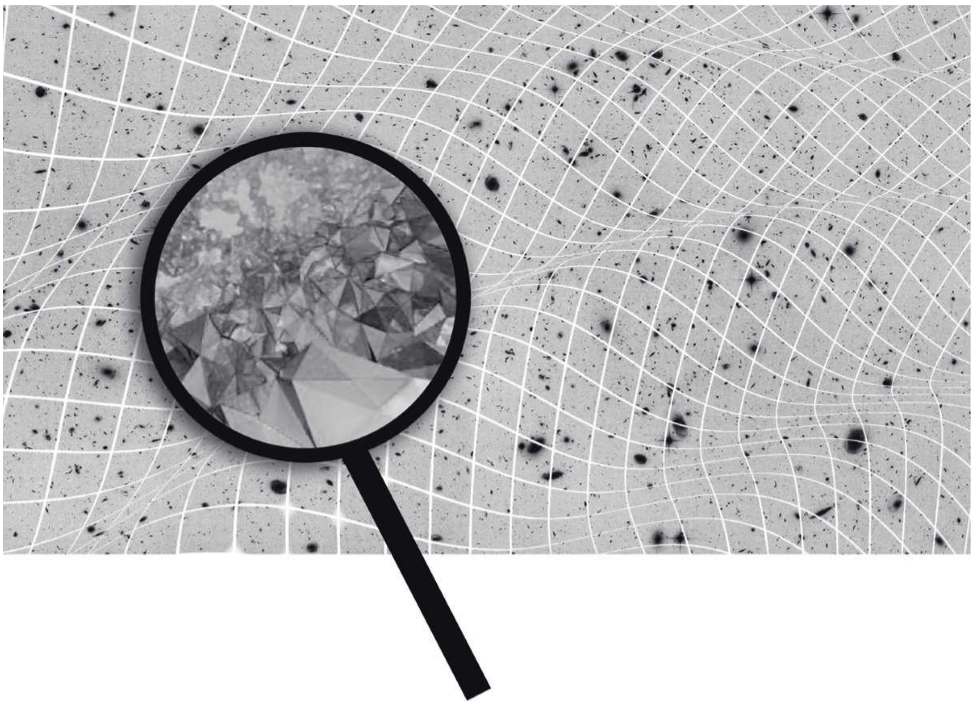
\includegraphics[width=3\textwidth]{img/51.png}\\[12pt]
\ec
\caption{我们在第三章已经见到这幅图像的背景了。没错,就是那张哈勃望远镜拍摄的宇宙图景基础加上表示弯曲空间的辅助线的图片。按照原文“通过甚强的放大镜,用考察极端的特写镜头”,我们便看到了放大镜中间的图像,也就是宇宙在极小尺度下的图像。对于化学或者材料稍微熟悉的人,规整的起伏和一些排列在一起的晶胞还是非常相像的;让这个比喻再通俗一点,就好像非常多盐的颗粒平整地撒在桌面上。在图像中,这些“晶胞”或者“颗粒”不是紧致的堆在背景当中,在近处它们聚在一起,但稍远处可以看到它们集束成多条纤维。通过这个细节,文章也展示了原文中不够形象的部分,比如,“‘环’组成了网状结构”和“像精细编织的巨大锁子匣一样,编织出了空间材质”。}
\label{fig:side:a}
\end{minipage}

\end{figure} 


    有可能实验验证这个理论吗?我们思考着尝试着,但是还没有实验的验证。无论如何,有一些不同的尝试。
    这些尝试中的一支派生出了
\href{http://toyhouse.cc/wiki/index.php/黑洞}{黑洞}
的研究。在天空中我们已经可以观察坍缩恒星形成的
\href{http://toyhouse.cc/wiki/index.php/黑洞}{黑洞}
。这些
\href{http://toyhouse.cc/wiki/index.php/恒星}{恒星}
被自身质量压碎,向自身塌陷,以及从我们的视野中消失。但是它去哪了?如果
\href{http://toyhouse.cc/wiki/index.php/圈量子引力论}{圈量子引力论}
是正确的,物质不可能真正探索到一个无穷的点上,因为不存在只有有限大小的宇宙块。在自身的重量下坍缩,物质一定会变得更加稠密,直到某个时刻,在这个时刻
\href{http://toyhouse.cc/wiki/index.php/量子力学}{量子力学}
一定会产生反作用的
\href{http://toyhouse.cc/wiki/index.php/平衡力}{平衡力}
。
    在假设的恒星生命的最后阶段就是人们所知的“普朗克星”。在这一阶段中时空量子涨落平衡了物质自身重量。如果太阳停止燃烧,形成一个
\href{http://toyhouse.cc/wiki/index.php/黑洞}{黑洞}
,黑洞直径将会有约一点五公里。在这个黑洞中心,太阳的物质将会继续坍缩,最终成为
\href{http://toyhouse.cc/wiki/index.php/普朗克星}{普朗克星}
。它的尺度就和那些原子的尺度差不多。太阳全部的物质被压缩进一个原子的空间:一个普朗克星应该是由这样极端状态的物质构成的。
    普朗克星不是不稳定的:一旦压缩到极限,它就会反弹,开始重新膨胀。这会导致一次黑洞爆炸。就像一个坐在黑洞中普朗克星上的假设观察者,这个过程将会是一个发生得极快的反弹。但是对于这个观察者,那些在黑洞外面的人时间不会以同样的速度流逝。同样的道理,在山上时间会比在海平面流逝得更快。除非她以外,因为极端条件,时间片段的差别是巨大的,并且对于恒星上观察者极快的反弹,对外面的人来说显得是在很长一段时间发生的事。这就是为什么我们观察黑洞总是在相当长时间中保持不变:黑洞是以看起来极端缓慢的动作正在反弹。
    有可能在第一批宇宙黑洞形成的大熔炉中,黑洞中的一部分正在爆炸。我们如果是正确的,就很可能观测到它们爆炸所激发出的,以来自太空高能宇宙射线形式的信号。这也允许我们观测和测量量子引力主导现象的直接效应。这是一个大胆的想法——它有可能失效,比如可能在原始宇宙没有形成足够多的黑洞,能让我们今天来探测它们的爆炸。但是这个信号的探索研究已经展开。我们将来会看到结果。
    这个理论的另一个结论,也是最壮观的结论之一,关系到宇宙的起源。我们知道怎样重建我们行星的历史,直到最初的,它还很小的时期。但是在那之前呢?对的,圈理论的方程允许我们回溯得更远,重建它的历史。
    我们可以发现当宇宙还极度压缩的时候,量子理论产生了斥力,导致了巨大的爆炸,“大爆炸”或者事实上是“大反弹”。事实上,我们的世界可能诞生自从,反弹之前的一个宇宙。这个宇宙在自身重力下坍缩到一个极小空间,正要重新膨胀,从而成为我们观测到的,身边正在膨胀的宇宙。
    在这个反弹的瞬间,宇宙坍缩进一个坚果壳内,是真正的量子引力的领域:时间和空间同时消失了,世界被溶化成一团集群的概率云。然而我们的方程依然能描述这个概率云。第五堂课的最终图景被转换成下图:

\begin{figure}[htbp]
\begin{minipage}[t]{0.3\linewidth}
\centering
\bc
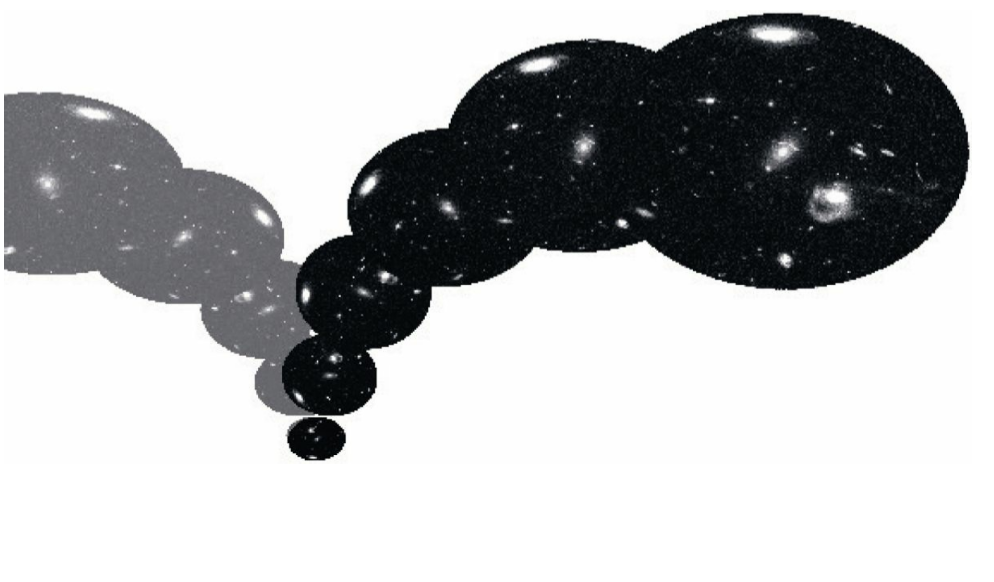
\includegraphics[width=3\textwidth]{img/52.png}\\[12pt]
\ec
\caption{可能在很多别的科普书中,我们看到过类似“实体”的右半支图像被用于形象描述我们的宇宙膨胀状态。在这里也概莫能外,事实上我们的宇宙也确实在加速膨胀。相对“虚”的,或者说有些透明的左半支则是一个相反的过程,宇宙的收缩状态。“虚”或者透明则是因为这是上一个宇宙对于现在的我们是不可观测的,目前我们没有任何手段能够预言并检测这个宇宙在反弹中的诞生之前的宇宙的任何有关讯息。}
\label{fig:side:a}
\end{minipage}

\end{figure} 

    我们的宇宙可能诞生自先前阶段的反弹,并经过一个既没有空间也没有时间的中间阶段。
    物理打开了一扇窗,从中我们可以看得很远,我们所见将会一直震惊我们。我们意识到,自身充满偏见,自身对世界的直觉图景也是偏颇的,狭隘的,也是不恰当的。世界不是平坦的,也不是静止的。世界将在我们眼前继续变化,我们逐渐能够将它看得更广阔,看得更清晰。如果我们尝试整理我们在二十世纪关于物理世界的所学,线索将会指向和我们对物质,空间和时间的直觉理解有深刻差异的事物上。圈量子引力论是一个企图破译这些线索的尝试,也是看向更远的一点距离的尝试。
\footnote[5]
{ 
作者本人也是圈量子引力论的提出者之一。
}


\noindent

		\chapter{概率、时间与\\黑洞的热}
\indent

    除了我已经讨论过的描述世界基本组成的主要理论以外,物理学仍然有一大堡垒与其他理论有所不同。一个简单的问题意想不到地产生了它:“什么是热?”

    截止到19世纪中叶时,物理学家们尝试着把热理解为一种叫做“
\href{http://toyhouse.cc/wiki/index.php/热质}{热质}
”的流体;或者是两种流体:一种热的,一种冷的。这个想法后来被证明是错误的。
\href{http://toyhouse.cc/wiki/index.php/詹姆斯·克拉克·麦克斯韦}{詹姆斯·麦克斯韦}
与奥地利物理学家
\href{http://toyhouse.cc/wiki/index.php/路德维希·玻尔兹曼}{路德维希·玻尔兹曼}
最终理解了热的本质。他们的解释十分奇特出众而影响深远——并且带领我们进入了很大程度上尚未被探索的领域。

    他们的研究表明一个有热量的物体并不包含任何热质。它不过是由运动更剧烈的
\href{http://toyhouse.cc/wiki/index.php/原子}{原子}
们所组成。原子与
\href{http://toyhouse.cc/wiki/index.php/分子}{分子}
以及束缚在一起的小型原子团不停地运动着。它们飞驰着、振动着、碰撞着……冷空气是由运动更缓慢的原子——或者说,分子——所构成的。而热空气是由运动更激烈的分子构成的。这个理论简洁而美丽,但却不止于此。

    正像我们所熟知的那样,热量总是从热的物体传向冷的物体。比如一个放在一杯热茶中的冷茶匙会变热,而我们不在气温低时多穿一点就会很快丧失我们身体的热量并感到寒冷。那么为什么热量会从热的物体传向冷的物体而不是相反呢?
\footnote[1]
{
作者开篇引出了热是什么这一问题?显然热对于我们来说是再平庸不过的日常触手可及的东西。可具体描述其又是相当具有难度的事情。事实上本章就要告诉大家热的这些特性与时间这一物理量有着密不可分的关系。
}

    这是一个关键的问题,因为这关系到时间的特性。在热量交换不发生或不明显的每个案例中,我们都能观察到系统的将来与过去十分相似。例如,热与太阳系中行星的运动几乎完全不相干,而事实上这样的运动可以反向的方式同等发生而不违反任何物理法则。然而,只要有热的存在,未来就不会与过去相同。比如说在没有
\href{http://toyhouse.cc/wiki/index.php/摩擦}{摩擦}
的情况下,摆锤会不停地摆下去。如果我们将其拍摄下来并将录像倒放,我们将会发现这运动是完全可能的。但是如果存在摩擦,那么摆锤将会极轻微地传热给它的支撑物并失去能量、缓慢减速:摩擦生热。而且我们能立刻分辨出未来(沿摆锤减速的时间方向)与过去的不同。我们从未见过一个从静止状态开始通过从支撑物吸收热进而摆动的摆锤。未来与过去的差别只有存在热时才会出现。这种基本物理现象借助热量由热的物体导向冷的物体实现了未来与过去的分离。

    那么,再一次的,为什么随着时间流逝热从热的物体传向冷的物体而不是相反呢?


    玻尔兹曼发现了这个简单得令人惊奇的原因:纯粹的
\href{http://toyhouse.cc/wiki/index.php/概率}{概率}
。

    玻尔兹曼的想法十分微妙,他引入了概率的理论。热并不是由于一条绝对的定律决定了它是由热的物体传向冷的物体的:热有如此的表现只是因为更大的可能性。这背后的原因是当一个处在较热物体中的快速移动的原子撞到一个较冷的原子时会更有可能传递给后者些许其自身的能量而不是相反。碰撞传递了能量但每次碰撞却并不同等地分配着能量。因此相互接触的物体的温度才会趋于一致。一个较冷物体接触较热物体使较热的物体升温是绝对不可能的。
    

\href{http://toyhouse.cc/wiki/index.php/概率论}{概率论}
向物理学核心的引入与在解释热动力学的基础方面,在其初期被认为是十分荒唐的。当时经常会看到没有人认真对待
\href{http://toyhouse.cc/wiki/index.php/玻尔兹曼}{玻尔兹曼}
的理论。1906.9.5,他在Trieste附近的Duino上吊自杀,永远也没有机会目睹他的理论收到普遍的承认。
\footnote[1]
{
玻尔兹曼的原子论曾被费曼如此评价:“假如在一次浩劫中所有的科学知识都被摧毁,只剩下一句话留给后代,什么样的语句可用最少的词汇包含最多的信息呢?我相信,这就是原子假说。”由此可见原子论对人类的重要性。然而当时的人们并没有意识到这一点。这导致了抑郁的玻尔兹曼的三次自杀,前两次自杀成功被人救下,最后一次却未能有人及时相救。遗憾的是,仅仅在其自杀两年之后,1908年,法国物理学家佩兰的实验最终判定了奥斯特瓦尔德“唯能论”的失败,奥斯特瓦尔德最后公开接受原子论。然而,玻尔兹曼已经没有办法亲眼见证自己理论的胜利了。
}

    在第二课中我将
\href{http://toyhouse.cc/wiki/index.php/量子力学}{量子力学}
如何预测每一小块物体的运动通过概率联系起来。这也将概率论放进了理论中央。但是玻尔兹曼考虑的关于热的本质的概率论与之有所不同。热力学中的概率在某种意义上与我们的无知紧密相连。

    也许我并不知晓有关
\href{http://toyhouse.cc/wiki/index.php/概率论}{概率论}
的相关内容,但我仍然可以确定某事发生的较小或较大的概率。例如,我不知道明天马赛港会下雨,也不会知道是晴天还是下雪,但是马赛港8月份下雪的概率很低。同样,对于大多数物体,我们有些许了解,但不完全知晓关于它们的状态的一切,我们只能根据概率进行预测。想象一个充满空气的气球。我可以测量它:测量它的形状、体积、压强、温度……但是气球内部的空气分子在其中快速移动,我不知道它们的确切位置。这阻止了我精确地预测气球的行为。例如,如果我解开这个结的封条,让空气流出,那他就会疯狂放气,左冲右突地让我无法预测他的位置。因为我只知道它的形状、体积、压力和温度,所以永远无法预测他放气状态下的位置。气球的运动取决于我无法了解的内部分子的碰撞。然而,即使我不能准确地预测每一件事,我也能预测一件事或另一件事发生的可能性。例如,气球几乎不可能会飞出窗外绕着远处的灯塔旋转,然后降落到我的手上,回到它被释放的那一点。有些行为发生的概率更大,而有些行为几乎不可能发生。

    同样,分子碰撞时热从较热的物体传递到较冷的物体的概率可以计算出比热向热物体传递的概率大得多。

    解释这些事实的科学分支被称为
\href{http://toyhouse.cc/wiki/index.php/统计物理学}{统计物理学}
。它的一个起自
\href{http://toyhouse.cc/wiki/index.php/玻尔兹曼}{玻尔兹曼}
的成果解释了热和温度的概率性——那就是
\href{http://toyhouse.cc/wiki/index.php/热力学}{热力学}
。

\footnote[3]
{玻尔兹曼提出了一个热力学基本常量,即玻尔兹曼常数。这里所说的成果应该是玻尔兹曼提出的关于单个气体分子的平均动能随热力学温度T变化的系数。其公式可以写为Ek=(3/2)kT。<br/>式中Ek为单个分子的平均动能,T为热力学温度。
}
 
   乍看之下,我们的无知昭示了物质的属性的想法似乎并不合理:热茶中的冷茶匙变热和气球被释放乱飞时。我们知道或不知道的事实与物理定律有什么关系?这个问题是合理的;而它的答案十分微妙。

    茶匙和气球的行为必须遵循完全独立于我们认知的物理定律。它们行为的可预测性或不可预知性与它们的精确状态无关;而与其相互作用的属性的概率有关。这组属性取决于我们与茶匙或气球相互作用的具体方式。概率并不是指物质本身的进化。它涉及到与我们相互作用的那些具体数量的演变。再次地,我们用来组织世界的概念的深刻的本质关系从中显现出来了。

    冷茶匙在热茶中加热是因为茶和勺子相互作用是通过描述它们微观状态的无数的变量中的有限变量下完成的。这些变量的值是不足以准确预测未来的行为(比如气球的飞行),但足以最佳可能的预测到勺子会被加热。

    我希望读者没有丧失对这些精妙的辨别的注重……

    现在,在二十世纪
\href{http://toyhouse.cc/wiki/index.php/热力学}{热力学}
(即关于热的科学)和
\href{http://toyhouse.cc/wiki/index.php/统计力学}{统计力学}
(即不同运动的概率的科学)的课程已经扩展到了电磁和量子现象。然而,包含引力场的扩展被证明是有问题的。重力场在加热时的行为如何,仍是一个尚未解决的问题。

    我们知道在加热的
\href{http://toyhouse.cc/wiki/index.php/电磁场}{电磁场}
中会发生什么:例如,在烤箱中有一种热电磁辐射可以烹饪馅饼,我们知道如何描述它。电磁波振动,随机的辐射能量,我们将所有的这团
\href{http://toyhouse.cc/wiki/index.php/光子}{光子}
想象为在一个热气球中运动的
\href{http://toyhouse.cc/wiki/index.php/分子}{分子}
。但是什么是热引力场呢?

\footnote[4]
{
我们再清晰的解释一下引力场到底是什么。相信大家对于牛顿被苹果砸的故事早已耳熟能详对于他的万有引力理论想必也早有耳闻了。引力场,是一种客观存在于空间的矢量场。对于标量的引力势求梯度可以得到引力强度。现在空间中测量得到的引力场,与利用广义相对论算得的该有的引力场值并不相同,人们认为这是因为空间中普遍存在一种,看不见摸不到但是却有质量的暗物质,这种物质提供了额外的引力,使得我们的世界成为了现有的样子。
}

    正如我们在第一节课中看到的,引力场即是空间本身。它影响时空。因此,当热量被扩散到重力场时,时间和空间本身必须振动……但我们仍然不知道如何很好的描述这个现象。我们没有方程来描述热时空的振动。以及什么是振动的时间?

    这些问题把我们带到时间问题的核心:时间的确切流向是什么?

    这个问题已经存在于古典物理学中,哲学家们在第十九、第二十世纪强调了这一点,但它在现代物理学中变得更为尖锐。物理学用公式来描述世界,它告诉我们事物如何随时间的变化而变化。但我们可以写下告诉我们事物如何关于位置改变的函数,亦或是食物的味道关于黄油数量改变的函数。但时间似乎是流动的,而黄油或空间的位置并不流动。它们之间的差别来自哪里呢?

    提出问题的另一种方法是问自己:什么是“现在”?我们说,只有现在的事物存在:过去不再存在,未来也不存在。但在物理学中,没有东西与“现在”这个概念相对应。比较“现在”和“这里”。这里指定说话者的位置:两个不同的人在这里指向两个不同的地方。因此“这里”是一个词,它的意思是什么是取决于说出他的人在哪里。这种话语的术语是“索引”。“现在”也指说出这个词的瞬间,也归类为“索引”。但是没有人会梦想说“存在于这里”,而不存在于此的事物并不存在。那么为什么我们说“现在”存在,而其他事物不存在?“现在”是客观存在的东西吗?“流动”,使事物“一个接一个地存在”,还是只是客观的,像“这里”?

    这似乎是一个深奥的心理问题。但在现代物理学中已成为一个热点问题,因为狭义相对论表明,“现在”这个概念也是主观的。物理学家和哲学家得出的结论是,时间的概念对于整个宇宙来说就是一个幻象,宇宙的“时间流”是一个不起作用的概括。当他的意大利朋友贝斯去世时,爱因斯坦写了一封感人的信给米歇尔的姐姐:“米歇尔已经一点点在我面前离开了这个陌生的世界。这不意味什么。像我们这样相信物理的人,知道过去、现在和未来之间的区别只不过是一种固执的甚至顽固的幻觉。

    幻想与否、是什么向我们解释了时间的流动与消逝呢?时间的流逝对我们所有人来说都是显而易见的:我们的思想和我们的语言都存在于时间之中;我们语言的结构需要时间——一件事物“是”或“曾是”或“将来是”。人们可以想象一个没有色彩的,没有物质的,甚至没有空间的世界,但很难想象一个世界没有时间。德国哲学家
\href{http://toyhouse.cc/wiki/index.php/马丁·海德格尔}{马丁·海德格尔}
强调了我们是“时间的栖居”。海德格尔对原始世界的描述是否有可能在世界的描述中消失?

    海德格尔的忠实哲学追随者们得出结论:物理学不能描述现实的最基本的方面,并将其视为一种误导性的知识形式。但很多时候,在过去我们已经意识到,我们眼前的直觉并不是准确的:如果我们依然笃信于此,我们将仍相信地球是平的,且太阳是围绕地球转的。我们的直觉是在我们有限的经验基础上发展而来的。当我们向前看得更远一点时,我们发现世界并不是像我们眼中看到的一样:地球是圆的,站在地球另一边的人,头是在下面的,脚是在上面的。仅仅相信眼前的直觉,而不是理性、谨慎和的整合性的审视,那是不明智的:在某些教条的老人的观念中,他是拒绝相信他村外的美好世界与他所知道的世界是有什么不同的。
\footnote[5]
{
这确实是一个复杂而又难以理解的问题。在现代的量子力学建立的过程中,“意识”这种神奇的东西一度成为人们争论的焦点。相信最著名的理论大概是“薛定谔的猫”了。实验是这样的:一只猫被关在一个密闭无窗的盒子里,盒子里有一些放射性物质。一旦放射性物质衰变,有一个装置就会使锤子砸碎毒药瓶,将猫毒死。反之,衰变未发生,猫便能活下来。按照量子力学的理论薛定谔的猫如果不观测时,竟然是既活又死的。也就是说,通过人们的意识作用可以决定猫的状态。这看起开是绝对不可能的事情。但是不妨如此理解,我们看到的世界其实不是我们看到的世界,是我们的意识告诉我们我们看到的世界是这样,所以我们才认为我们看到的世界是这样。可见意识可能并不是想我们想象中的是个“玄学”。
}

 
   正如我们所看到的那样生动,我们对时间流逝的体验不需要反映现实的一个基本方面。但如果它不是根本性的,我们对时间流逝的生动体验,它来自哪里呢?
 
   我认为答案在于时间和热量之间的紧密联系。只有在有热量流动的时候,过去和未来才会有可察觉的区别。热与概率有关,而概率又与我们与世界其他地方的相互作用不符合现实的细节有关。时间的流动是从物理学中产生的,而不是在对事物的精确描述的背景下。它出现在统计和热力学的背景下。这可能是时间之谜的钥匙。现在这个概念不存在比这里这个概念客观存在是更加客观的,但是,世间的微观作用导致出现了在只通过传递无数变量相互作用的系统(例如,我们自己)中的可见的现象。

    我们的记忆和意识是建立在这些统计上的现象。一个假设的超感官是不会有“流动”的时间:
\href{http://toyhouse.cc/wiki/index.php/宇宙}{宇宙}
是一个单块的过去,现在和未来。但由于我们意识的局限性,我们只能觉察到世界的模糊景象,并活在时间之中。借用我的意大利编辑的话:“不明显比明显的要多得多。”从这有限的、模糊的焦点中,我们可以看到时间的流逝。这样就清晰了吗?不,当然不。这里依旧还有很多东西需要去被理解。

    时间处于
\href{http://toyhouse.cc/wiki/index.php/引力}{引力}
、
\href{http://toyhouse.cc/wiki/index.php/量子力学}{量子力学}
和
\href{http://toyhouse.cc/wiki/index.php/热力学}{热力学}
交叉点引起的混乱的问题的中心。我们仍然有一系列问题依旧不明了。如果我们可能已经开始了解量子引力论,就会发现它结合了这三个谜题中的两个,但我们还没有一个理论能够把我们世界的三块基本知识结合起来。

    解决这个问题的一个小小的线索来自于物理学家
\href{http://toyhouse.cc/wiki/index.php/史蒂芬霍金|史蒂芬·霍金}{史蒂芬霍金|史蒂芬·霍金}
所完成的计算。尽管这位物理学家以被限制在轮椅上且不借助辅助器械无法发声的身体条件而出名,他依旧持续不断地钻研着物理。
\footnote[6]
{
这里指的1974年,霍金利用量子力学认真的研究了黑洞邻近的粒子行为后宣布黑洞具有温度,就像所有具有温度的物体一样,黑洞也能产生辐射!这种现象被称为霍金辐射。这里有段小插曲,上个世纪70年代,黑洞无毛定律被接受,意味着黑洞仅有质量、电荷和角动量三个参数,继而在1973年,霍金和另外两位物理学家合作写了一篇题为《黑洞的热力学定律》的论文,总结了与热力学定律相似的一系列关于黑洞的定律。该论文中着重强调了黑洞的温度为零(由于没人任何东西可以逃脱黑洞,因此它们不会辐射),并且不具有物理熵。但是,一位年轻的研究生雅各布·贝肯斯坦并不同意这个观点。他意识到如果黑洞不具备熵,热力学第二定律就会被违反。因为那样的话,我们就可以将任意具有熵的物体扔进黑洞,因此降低了外部宇宙的总熵。因此他认为黑洞的熵必须正比于表面积,才能挽救热力学第二定理。
}
 
   霍金利用
\href{http://toyhouse.cc/wiki/index.php/量子力学}{量子力学}
成功地证明
\href{http://toyhouse.cc/wiki/index.php/黑洞}{黑洞}
总是“热的”。它们像火炉一样散发热量。这是对自然中“热空间”的第一个明确提出。从来没有人观察到这种热,因为它在目前观测到的黑洞中是微弱的。但霍金的计算是令人信服的,它已被不同方式的验算所确证,黑洞的热的现在已被普遍接受。

    黑洞的热是物体上的量子效应,黑洞是自然界的引力。是单独的空间量子,空间的基本粒子,振动分子,加热了黑洞表面并产生黑洞热。这一现象涉及到量子力学、
\href{http://toyhouse.cc/wiki/index.php/广义相对论}{广义相对论}
和
\href{http://toyhouse.cc/wiki/index.php/热学}{热学}
这三个方面。黑洞的热就像物理学的
\href{http://toyhouse.cc/wiki/index.php/罗塞塔石碑}{罗塞塔石碑}
,用三种语言书写–
\href{http://toyhouse.cc/wiki/index.php/量子}{量子}
、
\href{http://toyhouse.cc/wiki/index.php/引力}{引力}
和
\href{http://toyhouse.cc/wiki/index.php/热力学}{热力学}
。它仍在等待着解读来揭示时间的本质。

\noindent

		\chapter{最后:我们自己}
\indent

    从深空的结构到所认知的宇宙边界我们已经遨游了如此遥远了。在这之后,在结束这系列课程致前,我想回归到“我们自己”这个主题上来。

    当代物理描绘出一幅关于这个世界的伟大壁画,在这物理学家所绘制的壁画中,我们作为感知者、决定者,能自由表达自己情感的人类,扮演了一个怎样的角色呢?如果世界是一群转瞬即逝的空间和物质的量子,如同一个空间和基本粒子的巨大拼图,那我们是什么呢?我们也仅仅是由
\href{http://toyhouse.cc/wiki/index.php/量子}{量子}
和
\href{http://toyhouse.cc/wiki/index.php/粒子}{粒子}
构成的吗?如果是这样,那么我们全部都能感知到的个体存在感和独特个性,又是从何得来的呢?我们的价值,我们的梦想,我们的感情,以及我们的个体知识究竟是什么?在这个漫无边界又光芒无限的世界中,我们又是什么呢?
\footnote[1]
{ 
作者此章开篇即抛出问题,我们是什么?这的确是一个值得我们思考的问题。这个深邃的问题,不禁让人堕入幻想的漩涡。悠远苍茫的声音在耳畔回响“天地玄黄,宇宙洪荒,日月盈昃,辰宿列张……”,自然万物皆有物理定律支配其运行,虽有量子力学般的不确定性,但总还可进行一定意义上的预测。可我们自己呢?谁能预测我们的未来?
}

    我甚至不能想象用这样简单的篇幅真正完美地回答这样一个深奥的问题。这是一个艰深的问题。在当代科学的巨大图景中,有很多我们暂时无法理解的事物。其中,我们最难以理解的一个就是我们自己。但若是回避或者忽略这个问题,我想,我们会遗漏某些关键性的事物。我已经着手于展示科学之光下的世界是何面貌,以及,作为这个世界的一部分的我们的面貌。

    我们,
\href{http://toyhouse.cc/wiki/index.php/人类}{人类}
,是第一个也是最重要的,观察世界的
\href{http://toyhouse.cc/wiki/index.php/主体}{主体}
;也是我所尝试组合的显示照片的集体作者。我们是图像、工具、信息的传递网络和知识的交换(本书就是一个例子)网络中的结点。

    但是我们也是我们所感知的世界的一个整体部分;我们不是外部的观察者而是也置身其中。我们对世界的认知来亦自其中。我们由像在山中构成松树的
\href{http://toyhouse.cc/wiki/index.php/原子}{原子}
,和群星间交换的光信号等同类物质所组成。

    随着我们知识的增长,我们已经认识到我们只是宇宙中微乎其微的很小的一部分。

    几个世纪以来,尤其是在上个世纪,这一点变得越来越明显。我们曾经相信我们生活在宇宙中心的星球上,事实证明我们错了。我们曾认为我们是一个特别的存在,一个独立于动植物的种族,然而后来发现我们是和身边一切生物有着共同祖辈的后代。我们和蝴蝶、落叶松有着共同的祖先。我们只是唯一一个长大了的孩子,唯一地认识到世界没有像小时候那样围绕着孩子们。人类必须学会融入众生中去。参照自然,参照其他的事物,并最终了解我们是谁。


    在德国
\href{http://toyhouse.cc/wiki/index.php/唯心主义}{唯心主义}
的全盛时期,
\href{http://toyhouse.cc/wiki/index.php/谢林}{谢林}
大概认为人性代表了了解自然的顶峰,最高点。今天,从我们现在对自然世界的知识提供的视点看,谢林的想法只会让我们呵呵一笑。即使我们与众不同,也只是每个人感到自己不同这般。这仅仅如同每个母亲都认为自己的子女与众不同。但是对于自然的其余部分,显然就不是这样了。

    在巨大星河中,我们偏居一隅;在构成现实的无限的不同样式的蔓藤花纹之中,我们只是无数我们这样点缀的其中一个。

    我们所构建的宇宙图景在我们思维空间中与我们俱生。我们重建如图片般能用浅薄手段理解的事物,在和我们作为一部分的现实世界之间,存在着无数的像“我们的无知,我们的感知和有限的智慧”般的马赛克筛子一样的东西。在这方面我们与作为这世界主体的大自然有着惊人的相似条件。

    这些条件,无论如何并不是
\href{http://toyhouse.cc/wiki/index.php/康德}{康德}
设想的是那样朴素(然而显然是错的)——从中推出自
\href{http://toyhouse.cc/wiki/index.php/欧几里得空间}{欧几里得空间}
的空间观甚至到牛顿力学的自然观这些皆注定是先验的。它们是我们种族精神演化的结果,是在连续的演化中的。我们不仅认识到,也渐渐认识到去改变我们理念框架,以使之适应于我们所认知。并且我们尽管缓慢犹豫,但一直在学习去认识到的,正是我们作为部分的现实世界的自然。我们建构宇宙的图景活在我们心中,在理念的空间中;但是他们也或多或少描述了我们所属的宇宙。我们为了更好地描述这个世界而遵循线索。
\footnote[2]
{
此段大部分使用意译的方法,其英语原文使用了大量难以翻译的从句手法,给翻译带来了许多困难。译者在尽量保持原文滋味的前提下对文章进行了微小地再创作。
}
\footnote[3]
{
总结而言,从这里开始,将在描述人类是认知“我们”自身的过程。这部分文字列举的对象,主要是欧洲的哲学家,但是作者也在很无情嘲讽他们的认知尚不完全。不过这里是基于现代人的观点而言的,在这里采用这样的行文方式,没有生涩的历史感,更容易让读者接受。
}

    当我们谈起“大爆炸”或者空间结构的时候,我们正在做的不是人们千百年来在篝火讲述自由奇幻的故事的延续而是别的东西的延续。在一天的第一抹晨曦中,我们看着羚羊在大草原翻飞的尘土中留下点点印记,我们通过仔细观察,从现实的细节中剔出那些无法直接看见的,但可以追寻踪迹的东西。在我们总会犯错因而时刻准备在新踪迹出现时转向的意识中,我们也同时在认识到如果我们做得足够好,我们最终会正确并找到我们一直所寻找的猎物。这就是科学的自然。

    在这两类人类活动——发明故事和按图索骥——中的困惑,就是在我们当代文化下展现出的对科学的不解和怀疑。这个分歧是个微妙的分歧:破晓时被猎捕的羚羊还未从在夜时故事会中的羚羊众神中远远剔除。

    二者的边界是互通的。神话滋养着科学,科学滋养着神话。但是,一旦我们发现了可以吃掉的一只羚羊,知识的价值将会留存。

    我们的知识持续的映射着世界。它或多或少,但的的确确反映了我们所栖息的世界。我们自身和世界的这个沟通,不是我们和自然的其余部分间的区分。一切事物都一刻不停地相互作用着,在作用中每个事物都产生着与其作用过的事物的痕迹:在这个意义上一切事物都一直在相互交换着信息。

    一个物理系统对另一个系统的信息对其而言没有任何精神性或者主观性:他仅仅是物理决定的一者和他者间的联系。一滴雨包含了天空中出现云的信息;一束光包含了其发射源的颜色;一个时钟有着一天的信息,风承载了将至的暴风的信息;流感承载了我鼻子易感性的信息;我们细胞中
\href{http://toyhouse.cc/wiki/index.php/DNA}{DNA}
包含了一切我们
\href{http://toyhouse.cc/wiki/index.php/基因}{基因}
编码的信息(在我和父母相像的意义上);以及我大脑充满我经历所积累的信息。我们思维的原始面目就是一个极端富集的信息。而且它在不断积累,交换并且娓娓道来。
 
   即使我中心供热系统的恒温器也“感知”并“知晓”我家的大气温度,并且拥有他的信息,可以在够热的时候自己关掉。所以,在温暖并自由决定关闭加热与否上,那恒温器的“感知”和“知晓”与我们的“感知”和“知晓”区别是什么?也“知晓”我的存在吗?到底自然中怎样的信息交换产生了我们和我们的思维?
\footnote[4]
{
用恒温器的例子来做隐喻是很形象的例子。从认知学的角度看,人认知的方法与恒温器认知的方法上似乎没有什么区别,那么我们独特的原因又在哪里呢,请读者认真思考,下文中将有详述。
}

    问题是开放的,有着无数在讨论之中的解答。我相信这是最有趣的科学前沿。在这里主要的过程就是关于被创造。今天新的工具允许我们观察到活跃大脑的活动,并且能够视听化地定位高度错综复杂的网络。正如2014年新闻所宣布的人类已完成首个哺乳动物的大脑结构的彻底(中观)详细定位。此外,对结构的数学形式可以对应于意识的主观体验的观点现在正在讨论中。这不仅仅是被哲学家讨论着,也正在被神经学家讨论着。

    举一个奇妙的例子,
\href{http://toyhouse.cc/wiki/index.php/朱利奥·托诺尼}{朱利奥·托诺尼}
——一位工作在美国的意大利科学家——发展了一个数学理论,被称为“积分信息理论”。它试图定性的分析出特征化具备意识系统的必要结构:作为例子的一个方法是,描述我们在清醒(有意识)和无梦睡眠(无意识)间到底发生了些什么变化。它仍然还在发展阶段。对于我们意识到底如何形成,我们仍然没有令人信服的,已经建立的答案。但对我而言,迷雾已经渐渐消散。

    有一个问题,特别是关于我们自己,常常让我们困惑的问题:如果我们的行为仅仅是预定的自然法则,那我们决定的自由意味着什么呢?我们自由感和如同我们现在所了解的,世间万物运行的严谨,这二者之间有没有可能不存在一个矛盾呢?我们内在可能有没有,这样一个东西,让逃离自然的规律,让我们用自由思考的力量去扭曲和偏离自然规律?

    好吧,答案是否。这里没有能让我们逃离自然法则的东西。如果我们内在存在着可以违背自然的某种事物,到现在我们可能早就发现它了。我们内在没有和事物的自然行为存在矛盾之处。整个现代科学——从物理到化学以及从生物到神经科学——只是仅仅证实了这种观
察。
 
   对这种困惑的答案到处都是。当我们说我们是自由的并且我们可能自由是真的,这就意味着我们如何行为是由我们内部,在大脑中发生的事物所决定的,而不仅仅是外部因素。是自由的不意味着我们的行为不受自然法则决定。这只是意味着它受我们大脑中活动的自然法则所决定。

    我们自由决定是由我们大脑中数亿
\href{http://toyhouse.cc/wiki/index.php/神经元}{神经元}
间的,丰富和流动的交互结果所决定:它们是自由的。从这些神经元所能允许和决定的交互的意义上来说是这样的。这可以意味着当我作决定,是“我”真正决定了?是的,当然。因为下面这个问题显得很荒诞。“我”到底能不能做与我整个复杂神经元所决定的不同的事物:这两者,如同荷兰哲学家
\href{http://toyhouse.cc/wiki/index.php/巴鲁奇·斯宾诺莎}{巴鲁奇·斯宾诺莎}
在十七世纪所清晰理解的一样,是完全相同的。

    单独的“我”和“大脑中的神经元”都是不存在的。它们是相同的东西。一个个体,就是一个进程:复杂的,高度集中的进程。

    当我们说人类行为不可预测的时候我们是对的,因为预测太过复杂,尤其是被我们自己预测。我们强烈的内在自由感,如同斯宾诺莎敏锐观察到的,来自于我们关于自生的想法和图景相比于我们内在发生的细节的复杂事物来说是远远地更加粗略的。我们就是我们自己眼中无尽惊奇的源头。

    我们大脑中有数百亿神经元,如同星系中的群星那样多。这些神经元甚至有着天文数字般更多的连接和可能组合。通过这些组合神经元可以相互作用。我们不可能意识到这全部。“我们”是由这复杂整体组成的进程,而不是其中使我们有意识的一小部分。
 
   决定的“我”就是自我反思构成(某种意义上仍然不完全清晰但是我们已经开始了解)的“我”;也是在世界中自我表达构成的“我”;也是自身理解为置于世界背景下的一个可变化的观察点的这种想法构成的“我”;也是大脑中处理信息组成表达的宏大结构构成的“我”。当我们已经感受到“这就是我”在做决定的时候,我们就是正确的。如果这不是我,那什么又是我呢?

    如同斯宾诺莎所维持的,我就是我的身体和发生在我心脑中的事物,也是对于我而言的巨大的不可思议的复杂性。

    涉及到这些篇幅的,我所拥有的科学的世界图景,不会和我们对自己的感知相矛盾。它也不会和道德或者心理学术语下我们的思维相矛盾,也不会和我们情绪和感受相矛盾。世界是复杂的,我们用不同语言去描述它,每个语言都与我们正在描述的进程相适宜。每个复杂进程可以在不同语言中和在不同层次下被定位和理解。这些丰富的语言交互相织也相互促进,就像这些进程本身一样。在我们对大脑生化学理解之下,对心理的研究变得更加复杂。使我们活跃的热情和情绪滋养着理论物理的研究。

    我们的道德价值,我们的情绪,我们的爱,不再那么缥缈地作为自然的一部分,缥缈地和动物所共享共享或者缥缈地被我们种族百万年来潜移默化的演变所决定。他们只是我们创造的复杂现实世界。我们的现实就是过去萦绕我们的眼泪和欢笑,感恩和无私,忠诚和背叛,以及平静。我们的现实世界有社会,有音乐激发的情绪,由我们共同构建的寻常知识组成的富集的交织的网络。所有的这些只是被我们描述的自同为“自然”的一部分。我们是自然的一个整体部分。我们就是一个有着无穷无尽变量的表达式中的自然。这就是我们从对于世界事物不断增长的认知中所学会的。
 
    使我们明确成为人类不表示我们和自然的分离;这是自同自然的一部分。这是发生在我们星球上的,在组合的无尽表达下,通过相互影响和部分之间信息和关联的交换,是这样的形式,谁知道有多少和其他的非凡的复杂事物存在着,在无尽的宇宙空间中,大概以我们所不可能想象的形式……有如此多的空间,以至于认为在平凡星系中的偏僻角落中存在某种独一无二特殊的事物,这种想法显得很幼稚。地球上的生命仅仅提供了宇宙中正发生的冰山一角。正是我们的灵魂本身是唯一一个如此小的例证。

    我们是一个自然地被好奇心驱动的种族,有许多同等富于好奇心的种族构成的一个群
\href{http://toyhouse.cc/wiki/index.php/物种}{物种}
(
\href{http://toyhouse.cc/wiki/index.php/属}{属}
)中唯一剩下的一个。我们中的其他种族已经灭绝了;有的像
\href{http://toyhouse.cc/wiki/index.php/尼安德特人}{尼安德特人}
,很近,大概三千年前灭绝。我们所属的是一群在非洲演化的种族,类似于有层级和好争吵的大猩猩——还甚至更像倭黑猩猩
,一种小的安静的,乐观平等,和混种的黑猩猩。一群能够为了探索新世界反复走出非洲的种族。而且他们走的很远:最终远,到
\href{http://toyhouse.cc/wiki/index.php/巴塔哥尼亚}{巴塔哥尼亚}
——并且最终远到月球。

    有好奇心不是对抗自然:只是我们的自然就是这样。
 
   十万年来我们种族离开了非洲。我们可能恰恰被这种好奇心驱使,学会看向甚至更遥远的彼方。在夜晚飞过非洲的航班上,我曾徜徉:这些遥远的走向北方开阔空间的先祖中的一位,可能会抬头望望天,想象着一个遥远的后代会飞去那里,会思考万物的自然,也会仍然被那个恰恰相同的好奇心驱动。

    我相信我们的种族不会延续很久。它不像是由那种东西构成。举个例子那种让乌龟能够延续并或多或少不被改变的存在上亿年。我们属于短命的种属。我们的亲戚都已经灭绝了。何况我们造成了伤害。我们导致的残酷的气候和环境不太可能放过我们。对于地球来说这些就像一些无关紧要的昙花一现,但是我不认为我们能够从它们中毫发无损地逃出生天——尤其是公众和政治观点倾向于忽略这些危险,就像我们在逃避把头埋进沙子里。我们可能是地球上仅存的对我们个人死亡不可避免有着感知的物种。我害怕很快我们就已经成为了唯一的将会看着自己集体灭亡或者自身文明消亡到来的物种。

    正如我们或多或少知道如何去处理个体的死亡,我们应该会处理我们文明的崩塌。这没有多大不同。并且这注定不是第一次发生。玛雅和克里特,包括它们在内的许多其他文明,都已经经历过了。我们生死如同星辰生死,都是个体性的也是集体性的。这就是现实。生对于我们来说是宝贵的。因为它转瞬即逝。并且正如
\href{http://toyhouse.cc/wiki/index.php/卢克莱修}{卢克莱修}
所写:“我们求生若饥,我们求生若渴。”(物性论第III卷,拉丁语第1084行)但是沉浸在创造我们指引我们的自然中,我们不是无家可归的,悬在两个世界,世界的部分但是仅仅部分属于自然的却追求别的事物的物种。不:我们就在家里。

    自然就是我们的家。在自然中就是在家里。这个奇怪的五彩斑斓的和令人令人震惊的世界,我们探索的世界——在这里空间颗粒化,时间不存在,事物无处不在——不是别的正是让我们对真正自我感到奇怪的东西。因为这是唯一我们自然的好奇心所揭示给我们关于的我们住所的东西。关于我们是什么构成的。我们是由构成万物一样的星辰构成的。当我们沉浸在痛苦之中或者当我们体验巨大的快乐的时候,我们不是别的我们只能是:我们世界的一部分。
 
   卢克莱修表达得很美好:
\begin{verse} 

我们都诞生自同一个天降的种子;\\
我们中所有人都有同样的父亲,\\
来自地球,这个喂养我们的母亲,\\
接受澄澈的雨滴,\\
从它们中养育繁茂的小麦\\
和茂密的树木,\\
和人类,\\
和野兽的种群,\\
提供所有滋养一切躯体的食物,\\
带来美好的生活\\
并生生不息...\\
(物性论第II卷,拉丁语第991-997行)
 
\end{verse} 
\footnote[5]
{
拉丁语原文为

...Denique caelesti sumus omnes semine oriundi;

omnibus ille idem pater est, unde alma liquentis

umoris guttas mater cum terra recepit,

feta parit nitidas fruges arbustaque laeta

et genus humanum, parit omnia saecla ferarum,

pabula cum praebet, quibus omnes corpora pascunt

et dulcem ducunt vitam prolemque propagant...

(De Rerum Natura,II,991-7)

这里的翻译转译自《Seven Brief Physics Lessons》的英文翻译。原文中第一行的意思是我们诞生自天空,而原书的英译文中的天空的种子更可能指雨滴,而非实际的天体。
原本意思中包含,父亲和天空是同位语,天空降下雨水滋养我们;而母亲和大地是同位语,大地接收这这些澄澈的雨滴。在转译中遗失了这部分含义。
}

    爱和诚实是我们自然的一部分。渴求了解更多,并继续学习也是我们自然的一部分。我们对世界的知识不断增长。
 
   这里是我们正在学习的前沿。于此燃烧着我们对知识的渴望。 他们在空间结构最微小的距离中,宇宙的起源中,时间的本质中,黑洞的现象中,以及我们自己思想过程的运作中。在这里,在我们所知道的边缘,与未知的海洋相接触,照亮了世界的奥秘和美丽。正是最令人叹为观止的地方。




\noindent


	% Appendixes ---------------------------------------------------------------
	%	 Title aligned right and in italics with chapter number
\iffalse
	\titleformat{\chapter}[block]{\raggedleft\itshape}{}
		{0pt}{\parbox{\linewidth}{\raggedleft\vspace*{1em}\Huge \chaptername~\thechapter: #1}}

	\appendix
	\renewcommand\chaptername{Appendix}
	\renewcommand{\theequation}{\Alph{chapter}.\arabic{equation}}
	\setcounter{equation}{0}    % reset counter
	\addtocontents{toc}{\protect\hrulefill\par}
	\input{app1.tex}
	\input{app2.tex}
	\input{app3.tex}
	\input{app4.tex}
	

	% Bibliography ---------------------------------------------------------------
	%    Title aligned right and in italics
	\titleformat{\chapter}[block]{\raggedleft\itshape}{}
		{0pt}{\parbox{\linewidth}{\raggedleft\vspace*{1em}\Huge#1}}

	\cleardoublepage
	\phantomsection
	\addcontentsline{toc}{chapter}{References}
	\renewcommand{\bibname}{References}
	\bibliography{}
	\bibliographystyle{alpha}
\fi
\end{document}
